\chapter{Experimental comparison}

In this chapter, we will experimentally compare the models presented in the previous chapter. We will describe the experimental setup for each job scheduling variant (JSSP, FJSP, DJSP) and interpret the results. 

\section{Experimental setup}

\subsection{Instances}

\subsubsection*{JSSP}

To compare models capable of solving JSSP, we obtained 242 benchmark JSSP instances and their best known solutions from \cite{jssp_benchmarks}. Each instance is a text file describing a JSSP instance using Taillard Specification \cite{taillard_specification}, where there are two numbers on the first line: the number of jobs $|\mathcal{J}|$ and the number of machines $|\mathcal{M}|$. Then, on the next $|\mathcal{J}|$ lines are operation processing times $p_{ij}$ with one line corresponding to one job. The next $|\mathcal{J}|$ lines describe on which machines should operations be processed \cite{jssp_benchmarks}. This text file is fed to each model, and the resulting schedule and makespan are obtained.  An example of Taillard's Specification is shown below \cite{jssp_benchmarks}.
\begin{verbatim}
    1   3
    6   7  5
    2   3  1    
\end{verbatim}
In this example, there is one job and three machines. The first operation has a processing time of 6 and is processed on the second machine. The second operation is processed on the third machine with a processing time of 7, and the last operation is processed on the first machine with a processing time of 5.
\par
Since FJSP models take only FJSP instances as an input, we reformulate each JSSP instance as the FJSP instance with $|\mathcal{M}_{ij}| = 1$, whose text representation will be described in the following subsection. 
\par
For each model and each JSSP instance, we run the experiment with 10 different seeds. Besides makespan, we are also interested in \textit{gap}, which is given by the following equation
\begin{equation}
    gap  = \frac{C - C_\text{best}}{C_\text{best}} \, ,
\end{equation}
where $C$ is the makespan produced by the model or PDR, and $C_\text{best}$ is the best-known makespan from the literature \cite{jssp_benchmarks}.
\par
We also separated JSSP instances into three categories based on the number of jobs. Instances with less than 20 jobs are \textit{"small"}, instances with at least 50 jobs are \textit{"large"}, and \textit{"medium"} otherwise.

\subsubsection*{FJSP}

To compare two models capable of solving FJSP presented in the previous chapter, we obtained 402 benchmark FJSP instances and their best known solutions from \cite{fjsp_benchmarks}. Each instance is again a text file, where on the first line are at least two numbers: the number of jobs, the number of machines, and the last number corresponding to the average number of machines per operation is optional. Then, the next $|\mathcal{J}|$ lines represent one job. The first number is the number of operations in that job; the second number is the number of machines $k$ that can process the first operation, and then there are $k$ pairs of numbers corresponding to the eligible machine and its processing time of the given operation. This is followed by the data for the second operation, and so on. An example of an FJSP instance is shown below.
\begin{verbatim}
    1   3
    3   1   2   6   1   3   7   1   1   5   
\end{verbatim}
This FJSP instance example has one job with three operations. The first operation can be processed only on the second machine, the second operation can only be processed on the third machine, and the last operation can only be processed on the first machine. This FJSP instance is the JSSP instance example described above reformulated as an FJSP instance.
\par 
This text file is then fed to the model, and we obtain the schedule and the makespan. Again, we repeat the experiment for each model and each FJSP instance with 10 different seeds.
\par
As in the case of JSSP, we separated FJSP instances into three categories based on the number of jobs in the same way. Instances with less than 20 jobs are \textit{"small"}, instances with at least 50 jobs are \textit{"large"}, and \textit{"medium"} otherwise.

\subsubsection*{DJSP}
To compare our extensions of JSSP models to DJSP presented in the previous chapter, we designed an experiment inspired by \cite{djsp_experiment_design}. We assume that there is a set of jobs known at the beginning. We then model the arrival of new jobs as a Poisson process, i.e., the arrival of two consecutive jobs follows an exponential distribution \cite{djsp_experiment_design}. We model the average arrival time as 
\begin{equation}
    \Delta t_\text{avg} = \frac{\mu_a}{U} \, ,
\end{equation}
where $\mu_a$ is the average processing time of all operations, and $U$ is a load factor of the dynamic job shop. We use $U = \{1,2,4 \}$ in the experiment. 
\par
To generate the set of known and arriving jobs, we take the JSSP benchmark instance, shuffle the order of jobs in the text file, and use the first half of the shuffled instance as known jobs and the rest as arriving jobs. Again, we repeat each experiment with 10 different seeds.

\subsection{Models}
\subsubsection{L2D}
Authors of \textbf{L2D} trained \textbf{L2D} on randomly generated JSSP instances \cite{zhang2020learning}. They trained multiple parameter sets to examine the ability of the \text{L2D} to generalize to bigger JSSP instances. Each parameter set was trained on random instances of constant size. From their GitHub repository \cite{github_l2d}, we obtained parameter sets trained on instances with size 6x6, 10x10, 15x15, 20x15, 20x20, 30x15, 30x20. Number of trainable parameters in each parameter set is 19458. In our experiments, we use each obtained parameter set. 
\par
In each parameter set, each $\text{MLP}^{(k)}$ has two hidden layers, each with 64 neurons. The action selection and the value prediction networks have two hidden layers, each with 32 neurons. In PPO, the clipping parameter was set to $\epsilon = 0.2$. Number of GIN layers was set to $K = 2$. Parameters update was done using Adam optimizer with learning rate $2\times10^{-5}$. For specific details of the training process, we refer the reader to the supplementary material of \cite{zhang2020learning}.

\subsubsection{Wheatley}
For the experiment, we had to train \textbf{Wheatley} ourselves. To make \textbf{Wheatley} as similar to \textbf{L2D} as possible, we chose the same training hyperparameters as \text{L2D}. \textbf{Wheatley} has one extra training Hyperparameter specifying the maximum number of jobs and machines that the model will be able to process. 
\par
We trained three parameter sets capable of solving JSSP and one capable of solving DJSP. The first parameter set was trained on randomly generated 30x20 instances, capable of solving instances of size up to 100x20. The second parameter set was trained on randomly generated 20x20 instances, capable of solving instances of size up to 100x20. The last third parameter set was trained on randomly generated 20x20 instances and is able to solve instances of size up to \textbf{100x70} because, as discussed in \ref{dynamicwheatley}, for each arriving job, we add a new machine. And since the maximum number of jobs is 100, and half of them will be known at the start, we will have at most 70 machines. As a result, we used only the last parameter set for DJSP.
\par
The listed parameter sets were trained using a CPU on an Arm-based Ampere A1 virtual machine with 4 CPUs and 24 GB of RAM in Oracle Cloud Infrastructure with Ubuntu 20.04 64-bit operating system. We stopped the training when the model had not improved its objective for at least two days. Training of each parameter set took at least 3 weeks.

\subsubsection{IEEE-ICCE-RL-JSP}
Authors of \textbf{IEEE-ICCE-RL-JSP} trained the model on randomly generated 3x3 and 10x10 JSSP instances. Parameter updates are done using Adam optimizer with a $10^{-5}$ learning rate. As PDRs for agents to select in each step, we used FIFO, MOR, SPT, and MWKR discussed in \ref{priority dispatching rules}, the same choice as the authors made. The number of layers in HGIN was set to $K=3$. The value network has three dense layers. All hidden layers in both networks have dimension 128.
\par
No parameter sets were found in the GitHub repository\cite{github_ieee_icce_rl_jsp}, so we had to train our own parameter sets using a script found in the repository. The script trains the model until the \textit{gap} between the best-known solution and the solution given by the model is not smaller than 20$\%$. We trained five parameter sets. We trained the model using CPU on an Arm-based Ampere A1 virtual machine with 4 CPUs and 24 GB of RAM in Oracle Cloud Infrastructure with Ubuntu 20.04 64-bit operating system.

\subsubsection{End-to-end-DRL-for-FJSP}
Authors of \textbf{End-to-end-DRL-for-FJSP} trained the model on randomly generated instances with sizes 6x6, 10x10, 15x15, 20x10, 20x20, and 30x20. The number of GIN layers was set to $K = 2$. Each GIN layer has MLP with two hidden layers with dimension 128 \cite{LEI2022117796}. Job operation action selection decoder, machine action selection decoder, and state-value function all have two hidden layers with dimension 128. Adam optimizer with learning rate $10^{-3}$ was used to update the policy.
\par
We obtained only one parameter set from the GitHub repository \cite{github_end_to_end_drl_for_fjsp}.

\subsubsection{fjsp-drl}
Authors of \textbf{fjsp-drl} trained the model on randomly generated instances with sizes 10x5, 20x5, 15x10, and 20x10 \cite{9826438}. The model was evaluated on instances with a size of 30x10 and 40x10. The number of HGNN layers was set to $K = 3$, and the dimensions of operation and machine embeddings were set to 8. Five networks $\text{MLP}_{\theta_i}$ have two hidden layers with dimension 128, actor-network $\text{MLP}_\omega$ has two hidden layers with hidden dimension 64, and critic network also has two hidden layers with dimension 64. Hyperparameters for PPO were set to $I = 1000$ and $B = 20$. Adam optimizer with learning rate $2x10^{-4}$ was used for policy optimization. The discount factor was set to 1.0.
\par
We obtained five parameter sets from the GitHub repository for this model \cite{github_fjsp_drl}.

\subsection{Baselines}
We also compared previously described models with PDRs.
\par
\subsubsection*{JSSP}
For JSSP, we used PDR implementations from the code of the model \textbf{IEEE-ICCE-RL-JSP}. On top of FIFO, MOR, SPT, and MWKR discussed in \ref{priority dispatching rules}, we also used the following PDRs available in the code of \textbf{IEEE-ICCE-RL-JSP} \cite{github_ieee_icce_rl_jsp}:
\begin{enumerate}
    \item \textit{EDD} (Earliest Due Date)
    \item \textit{LOR} (Least Operations Remaining)
    \item \textit{LPT} (Longest Processing Time)
    \item \textit{LS} (Least Slack)
    \item \textit{SRPT} (Shortest Remaining Processing Time)
\end{enumerate}

\subsubsection*{FJSP}
For FJSP, we used PDR implementations from the code of the model \textbf{End-to-end-DRL-for-FJSP}. For operation selection, besides FIFO, we used three PDRs available in the code:
\begin{enumerate}
    \item \textit{MOPNR} (Most Operation Number Remaining)
    \item \textit{LWKR} (Least Work Remaining)
    \item \textit{MWKR} (Most Work Remaining)
\end{enumerate}
After selecting the operation, we used two machine selection PDRs available in the code:
\begin{enumerate}
    \item \textit{SPT} (Shortest Processing Time)
    \item \textit{EET} (Earliest End Time)
\end{enumerate}
All eight different combinations are used as baselines.

\section{Results}
We ran all experiments on a MacBook Pro with an Apple M2 Max chip, 32 GB of RAM, and Sonoma 14.4.1 macOS operating system. Besides reporting makespan and gap, we also report runtime for each experiment. 

\subsection{JSSP} \label{results_jssp}
Average gaps for different models and instance categories are shown in Table 4.1. The model with the lowest average gap is highlighted in bold. Average runtimes are in Table 4.2. 

\begin{table}
    Table 4.1: Average JSSP gaps for different models and categories\\
    \vspace{1mm}
    \small 
    \begin{tabular}{lllll}
        \toprule
        Model / Category & large & medium & small & all \\ 
        \midrule
        EDD & 0.30 ± 0.09 & 0.44 ± 0.11 & 0.35 ± 0.13 & 0.36 ± 0.12 \\
        FIFO & 0.28 ± 0.18 & 0.33 ± 0.11 & 0.25 ± 0.09 & 0.30 ± 0.13  \\
        LOR & 0.35 ± 0.09 & 0.44 ± 0.11 & 0.36 ± 0.12 & 0.40 ± 0.11\\
        LPT & 0.42 ± 0.11 & 0.48 ± 0.11 & 0.36 ± 0.10 & 0.44 ± 0.11\\
        MWKR & 0.19 ± 0.13 & 0.27 ± 0.11 & 0.17 ± 0.08 & 0.22 ± 0.12 \\
        LS & 0.24 ± 0.10 & 0.34 ± 0.09 & 0.31 ± 0.14 & 0.29 ± 0.11 \\
        MOR & 0.26 ± 0.20 & 0.28 ± 0.12 & 0.20 ± 0.08 & 0.26 ± 0.14 \\
        SPT & 0.22 ± 0.07 & 0.30 ± 0.08 & 0.24 ± 0.10 & 0.26 ± 0.09 \\
        SRPT & 0.35 ± 0.09 & 0.46 ± 0.11 & 0.39 ± 0.11 & 0.40 ± 0.11 \\
        End-to-end-DRL-for-FJSP & 0.28 ± 0.18 & 0.33 ± 0.12 & 0.30 ± 0.14 & 0.30 ± 0.14  \\
        fjsp-drl & 0.20 ± 0.15 & 0.25 ± 0.11 & 0.16 ± 0.08 & 0.22 ± 0.12 \\
        \textbf{IEEE-ICCE-RL-JSP} & \textbf{0.18 ± 0.13} & \textbf{0.24 ± 0.09} & \textbf{0.16 ± 0.07} & \textbf{0.20 ± 0.12} \\
        L2D & 0.28 ± 0.19 & 0.35 ± 0.12 & 0.25 ± 0.11 & 0.31 ± 0.16 \\
        Wheatley & 0.79 ± 0.59 & 0.43 ± 0.18 & 0.26 ± 0.11 & 0.48 ± 0.38 \\
        \bottomrule
    \end{tabular}
\end{table}


\begin{table}
    Table 4.2: Average JSSP runtimes for different models and categories\\
    \vspace{1mm}
    \label{table:4.2}
    \small
    \begin{tabular}{lllll}
        \toprule
        category & large & medium & small & all \\
        model &  &  &  &  \\
        \midrule
        EDD & 8.13 ± 7.10 & 0.75 ± 0.62 & 0.06 ± 0.05 & 4.04 ± 6.11 \\
        FIFO & 4.99 ± 5.67 & 0.70 ± 0.61 & 0.06 ± 0.05 & 1.69 ± 3.51 \\
        LOR & 3.26 ± 3.70 & 0.47 ± 0.40 & 0.04 ± 0.04 & 1.09 ± 2.26 \\
        LPT & 3.84 ± 4.20 & 0.70 ± 0.51 & 0.06 ± 0.05 & 2.20 ± 3.39 \\
        MWKR & 5.00 ± 4.86 & 0.60 ± 0.49 & 0.05 ± 0.04 & 2.31 ± 3.82 \\
        LS & 4.76 ± 4.72 & 0.52 ± 0.44 & 0.04 ± 0.03 & 2.43 ± 3.88 \\
        MOR & 3.83 ± 4.18 & 0.53 ± 0.46 & 0.05 ± 0.04 & 1.26 ± 2.58 \\
        SPT & 3.71 ± 4.20 & 0.60 ± 0.47 & 0.06 ± 0.04 & 2.10 ± 3.37 \\
        SRPT & 4.86 ± 4.58 & 0.46 ± 0.39 & 0.05 ± 0.03 & 2.41 ± 3.82 \\
        End-to-end-DRL-for-FJSP & 10.90 ± 11.96 & 1.74 ± 1.14 & 0.36 ± 0.20 & 4.97 ± 8.69 \\
        fjsp-drl & 49.13 ± 65.99 & 7.69 ± 5.22 & 1.14 ± 0.90 & 16.70 ± 38.10 \\
        IEEE-ICCE-RL-JSP & 16.26 ± 14.29 & 3.74 ± 2.16 & 0.58 ± 0.29 & 9.85 ± 12.17 \\
        L2D & 4.45 ± 3.99 & 1.10 ± 0.54 & 0.26 ± 0.14 & 2.46 ± 3.18 \\
        Wheatley & 32.34 ± 42.37 & 5.02 ± 3.56 & 0.89 ± 0.56 & 10.98 ± 24.60 \\
        \bottomrule
        \end{tabular}        
\end{table}

A boxplot for JSSP gaps for small instances is shown in Figure 4.1, for medium instances in Figure 4.2, for large instances in Figure 4.3, and for all instances in Figure 4.4. The model with the lowest average gap is highlighted as a blue box.

\begin{center}
    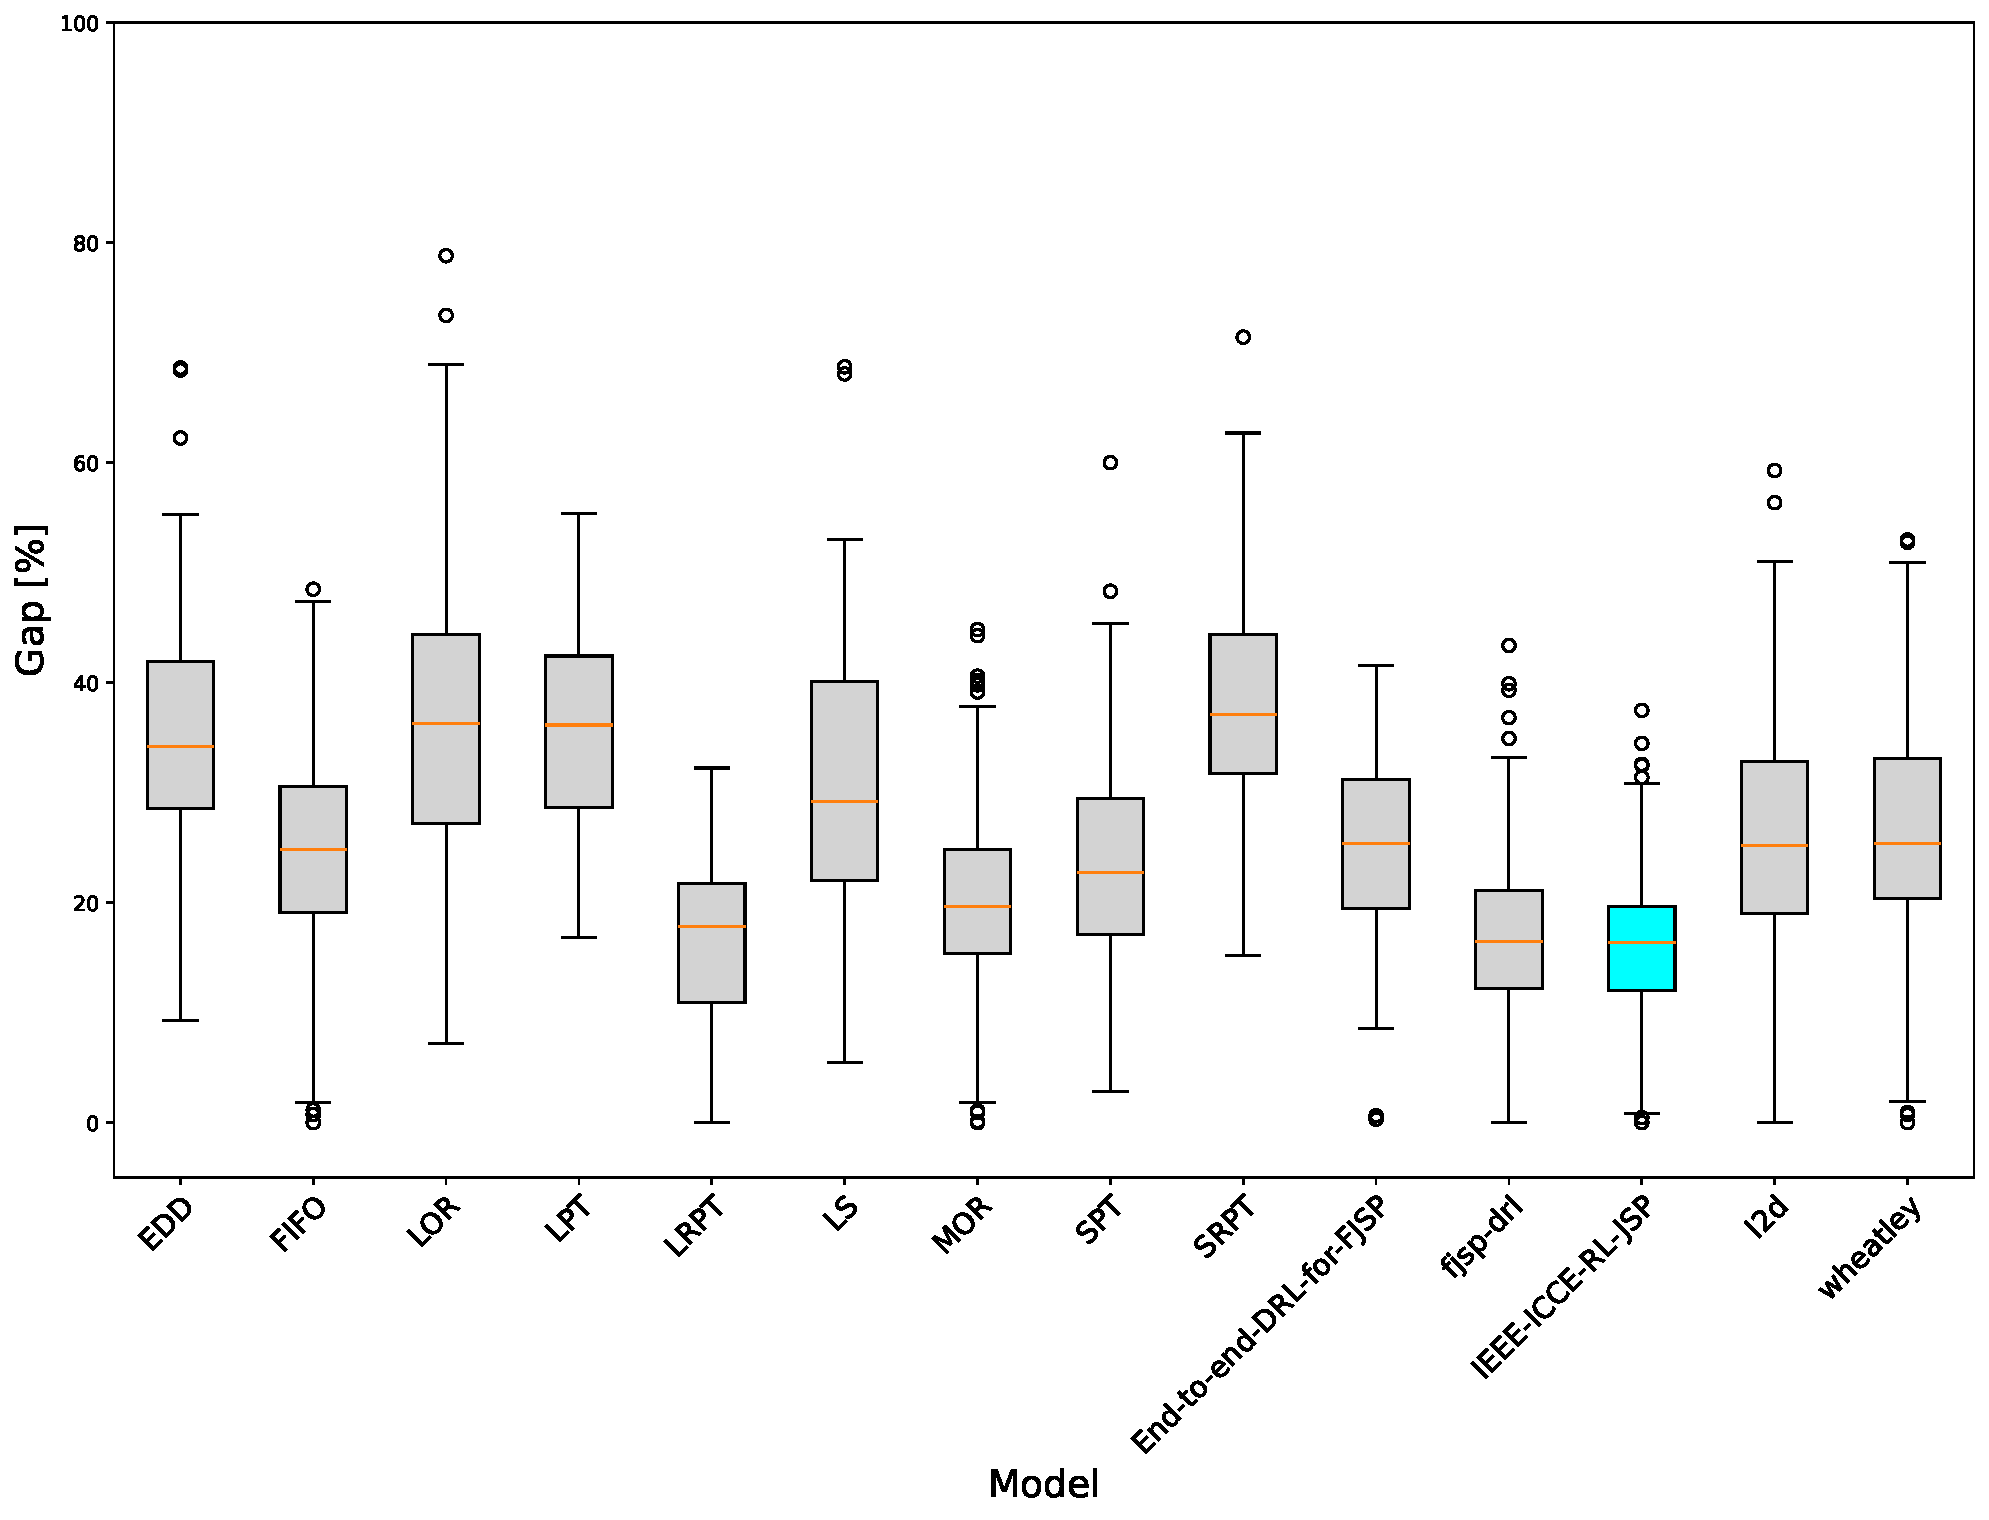
\includegraphics[width=0.8\linewidth]{images/horizontal_boxplot_jssp_small.pdf}\\
    Figure 4.1: JSSP gaps for small instances
\end{center}

\begin{center}
    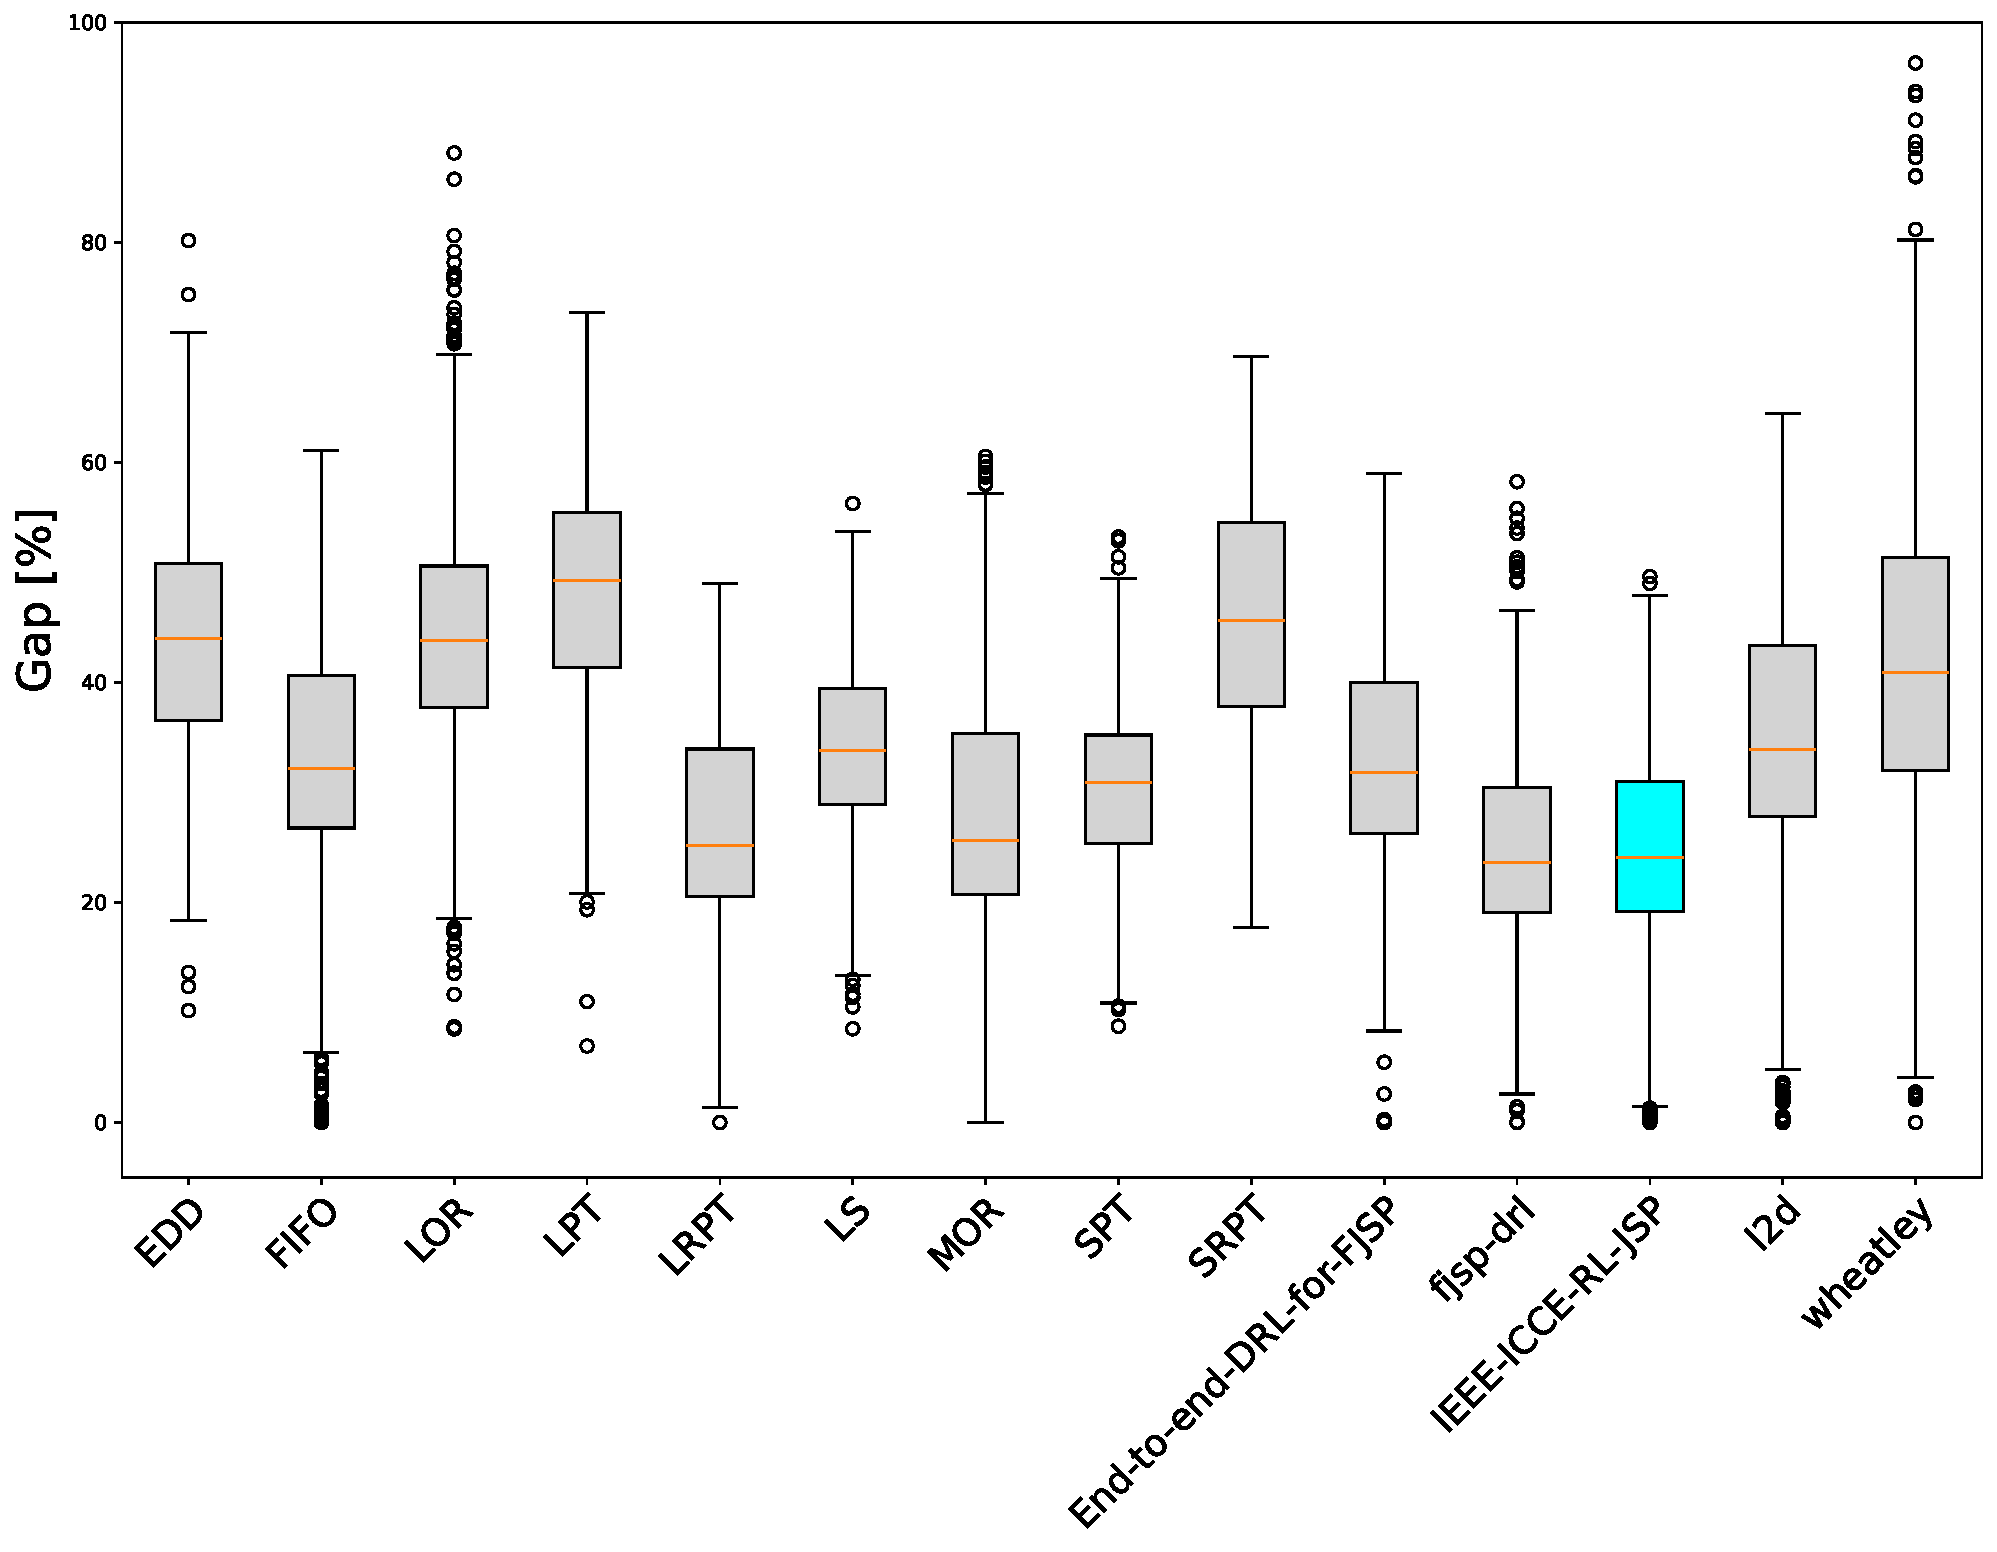
\includegraphics[width=0.8\linewidth]{images/horizontal_boxplot_jssp_medium.pdf}\\
    Figure 4.2: JSSP gaps for medium instances
\end{center}
\begin{center}
    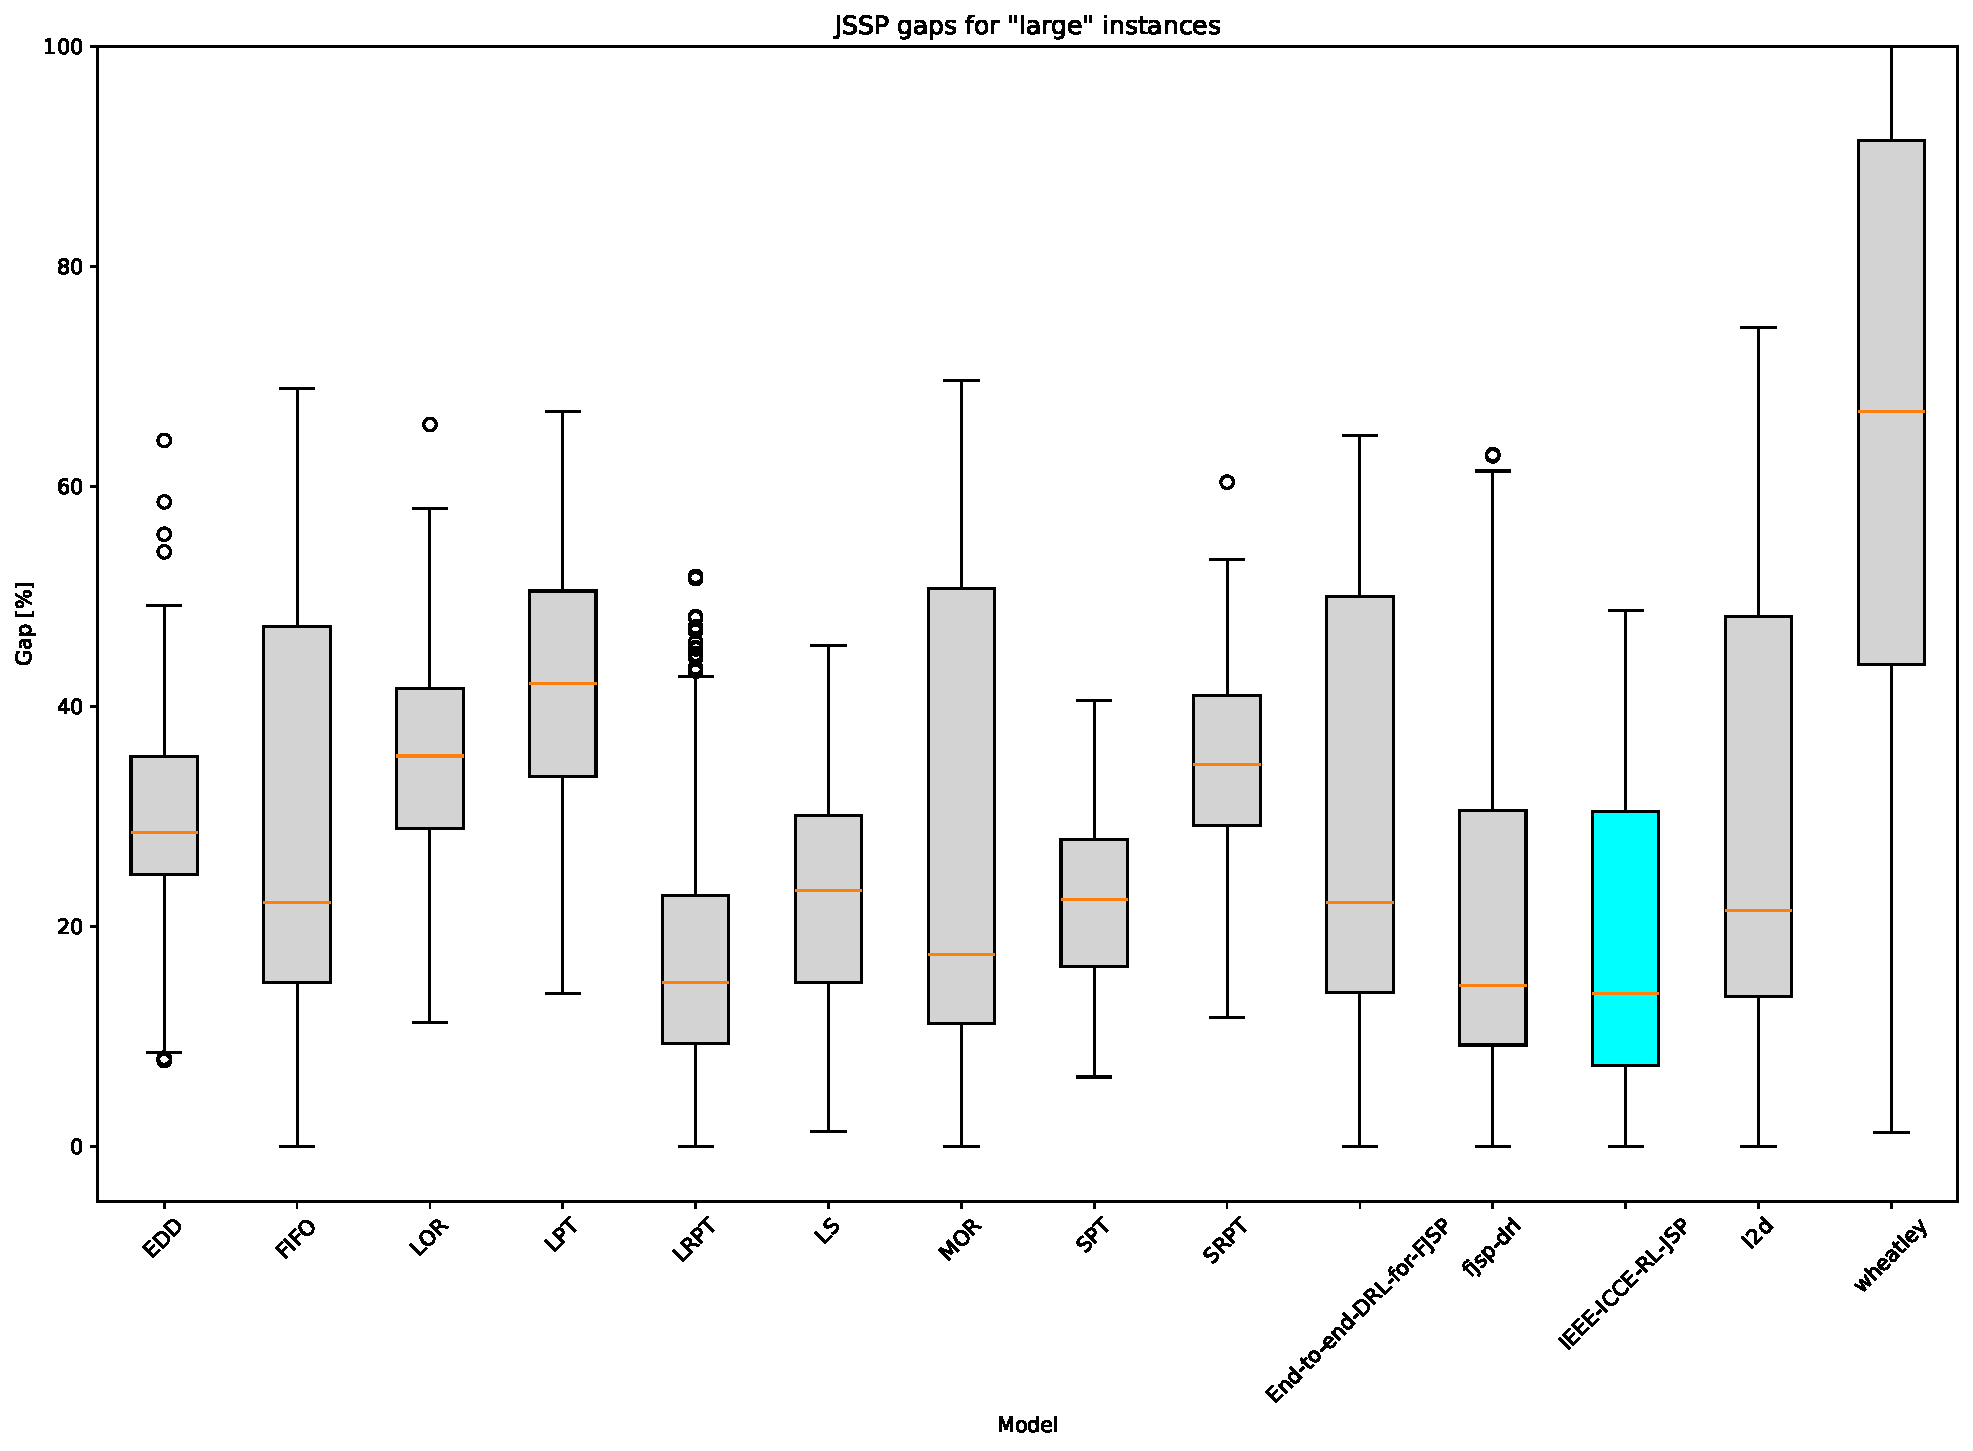
\includegraphics[width=0.8\linewidth]{images/horizontal_boxplot_jssp_large.pdf}\\
    Figure 4.3: JSSP gaps for large instances
\end{center}
\begin{center}
    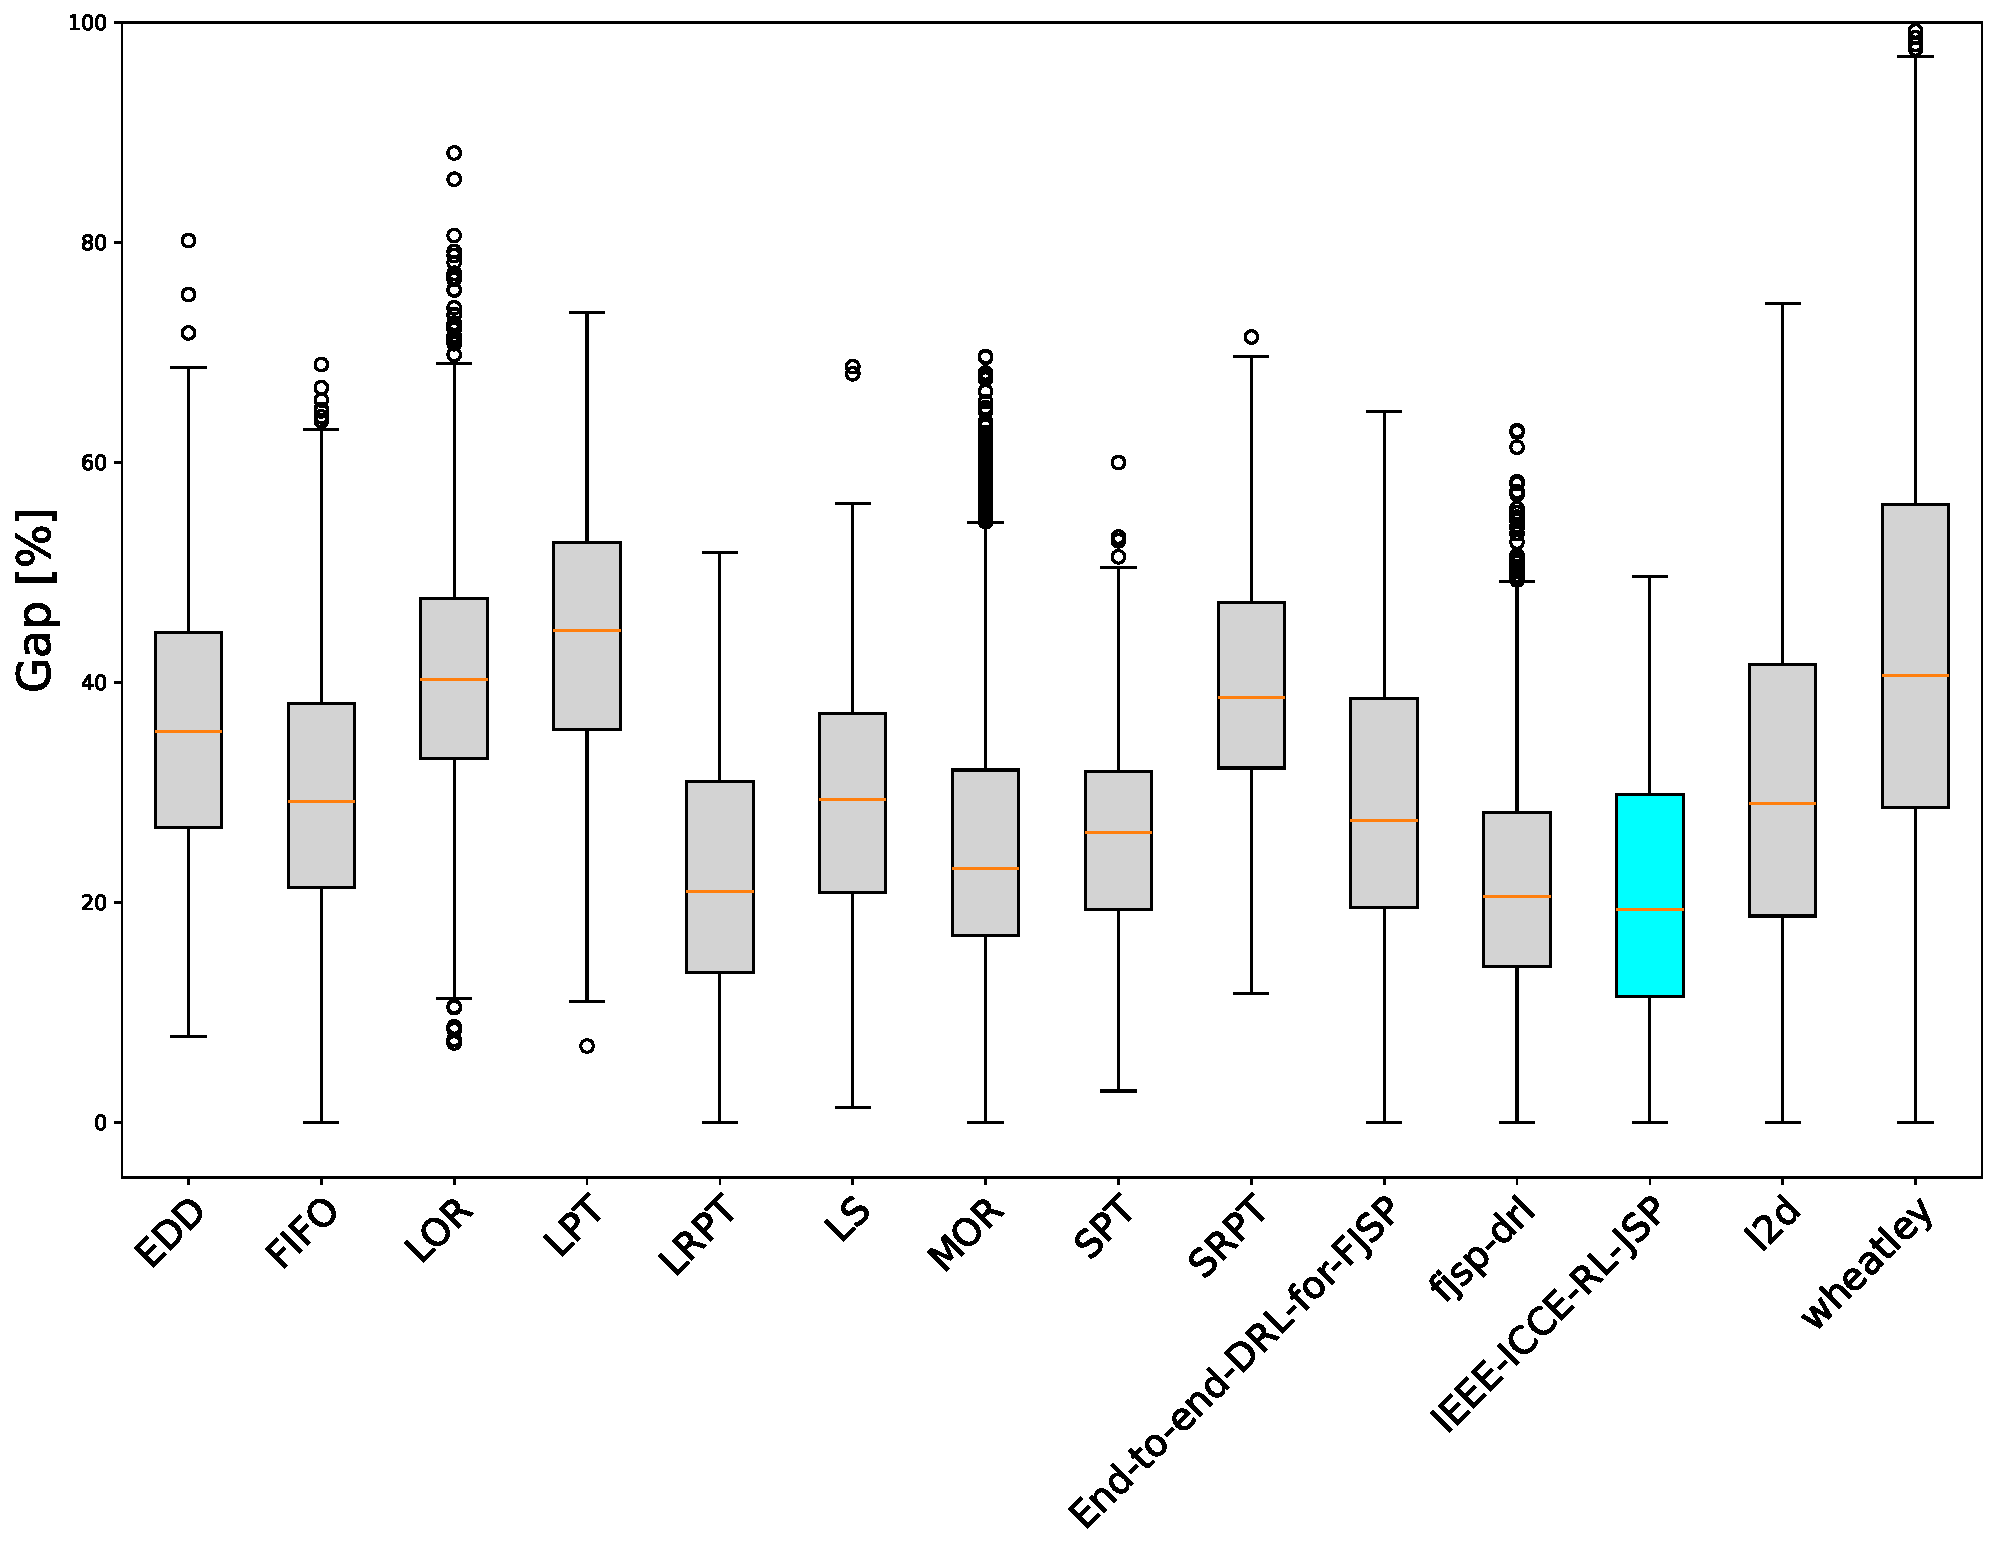
\includegraphics[width=0.8\linewidth]{images/horizontal_boxplot_jssp_all.pdf}\\
    Figure 4.4: JSSP gaps for all instances
\end{center}

To test the null hypothesis that the median values of all models and PDRs are from the same population, we used the Kruskal-Wallis test \cite{doi:10.1080/01621459.1952.10483441}. The p-value for JSSP gaps, including all models and PDRs in Table 4.1, is $p < 1\%$ for all sizes. We, therefore, reject the null hypothesis that all models and PDRs are equal. Without PDRs, the p-value is also $p < 1\%$. We reject the null hypothesis that all models are equal, too.
\par  
From Table 4.1 and Figures 4.1, 4.2, 4.3, and 4.4, we observed that priority dispatching rule \textbf{MWKR} and model \textbf{fjsp-drl} produced similar results as the model \textbf{IEEE-ICCE-RL-JSP}, which had the lowest mean gap. Therefore, we tested the null hypothesis that \textbf{MWKR}, \textbf{fjsp-drl}, and \textbf{IEEE-ICCE-RL-JSP} are from the same population. The p-value for small instances is $45.8\%$, for medium instances $1.1\%$, $3.8\%$ for large instances, and 0.1$\%$ for all instances. We, therefore, reject the null hypothesis that these three models are from the same population for medium and large instances.
For each pair of these three models, we then tested the null hypothesis using the Mann-Whitney \textit{U} test: that the pair of models was equal. Obtained p-values are shown in Table 4.3.

\begin{table}
    Table 4.3: p-values for Mann-Whitney \textit{U} test between pairs of models\\
    \vspace{1mm}
    \label{table:4.3}
    \begin{tabular}{llr}
    \toprule
    Category & Models & p-value \\
    \midrule
    large & MWKR + fjsp-drl & 85.1$\%$ \\
    large & MWKR + IEEE-ICCE-RL-JSP & 3.0$\%$ \\
    large & fjsp-drl + IEEE-ICCE-RL-JSP & 10.8$\%$ \\
    medium & MWKR + fjsp-drl & 0.6$\%$ \\
    medium & MWKR + IEEE-ICCE-RL-JSP & 0.4$\%$ \\
    medium & fjsp-drl + IEEE-ICCE-RL-JSP & 61.6$\%$ \\
    small & MWKR + fjsp-drl & 48.3$\%$ \\
    small & MWKR + IEEE-ICCE-RL-JSP & 22.7$\%$ \\
    small & fjsp-drl + IEEE-ICCE-RL-JSP & 48.0$\%$ \\
    all & MWKR + fjsp-drl & 48.3$\%$ \\
    all & MWKR + IEEE-ICCE-RL-JSP & 22.7$\%$ \\
    all & fjsp-drl + IEEE-ICCE-RL-JSP & 48.0$\%$ \\
    \bottomrule
    \end{tabular}
\end{table}

\subsection{FJSP}

Average gaps for different model and instance categories are shown in Table 4.4. The model with the lowest average gap is highlighted in bold. Average runtimes for different models and instance categories are shown in Table 4.5. A negative gap means that the model found a better solution than the one listed in \cite{fjsp_benchmarks}.

\begin{table}
    Table 4.4: Average FJSP gaps for different models and instance categories\\
    \vspace{1mm}
    \label{table:4.4}
    \footnotesize 
    \begin{tabular}{lllll}
        \toprule
        category & large & medium & small & all \\
        model &  &  &  &  \\
        \midrule
        FIFO-EET & 3.03 ± 0.23 & 0.54 ± 0.86 & 0.44 ± 0.96 & 0.67 ± 1.13 \\
        FIFO-SPT & 0.06 ± 0.12 & 0.37 ± 0.20 & 0.41 ± 0.22 & 0.37 ± 0.22 \\
        LWKR-EET & 3.09 ± 0.22 & 0.98 ± 0.83 & 0.91 ± 1.02 & 1.10 ± 1.10 \\
        LWKR-SPT & 0.15 ± 0.14 & 0.64 ± 0.28 & 0.71 ± 0.29 & 0.64 ± 0.32 \\
        MOPNR-EET & 3.63 ± 0.29 & 0.81 ± 1.11 & 0.72 ± 1.16 & 0.97 ± 1.35 \\
        MOPNR-SPT & 0.16 ± 0.15 & 0.39 ± 0.20 & 0.44 ± 0.22 & 0.40 ± 0.22 \\
        MWKR-EET & 3.18 ± 0.21 & 0.68 ± 0.96 & 0.57 ± 0.91 & 0.80 ± 1.13 \\
        MWKR-SPT & 0.17 ± 0.15 & 0.39 ± 0.18 & 0.43 ± 0.21 & 0.40 ± 0.21 \\
        \textbf{End-to-end-DRL-for-FJSP} & \textbf{-0.02 ± 0.09} & \textbf{0.17 ± 0.09} & \textbf{0.20 ± 0.11} & \textbf{0.13 ± 0.13} \\
        fjsp-drl & 0.26 ± 0.13 & 0.17 ± 0.18 & 0.22 ± 0.41 & 0.21 ± 0.35 \\
        \bottomrule
    \end{tabular}
\end{table}

\begin{table}
    Table 4.5: Average FJSP runtimes for different models and instance categories\\
    \vspace{1mm}
    \label{table:4.5}
    \footnotesize 
    \begin{tabular}{lllll}
        \toprule
        category & large & medium & small & all \\
        model &  &  &  &  \\
        \midrule
        FIFO-EET & 0.79 ± 0.47 & 0.14 ± 0.09 & 0.05 ± 0.05 & 0.13 ± 0.24 \\
        FIFO-SPT & 0.75 ± 0.45 & 0.14 ± 0.09 & 0.05 ± 0.05 & 0.13 ± 0.23 \\
        LWKR-EET & 0.64 ± 0.37 & 0.15 ± 0.09 & 0.05 ± 0.05 & 0.12 ± 0.20 \\
        LWKR-SPT & 0.65 ± 0.38 & 0.15 ± 0.09 & 0.05 ± 0.05 & 0.12 ± 0.20 \\
        MOPNR-EET & 0.67 ± 0.39 & 0.15 ± 0.09 & 0.05 ± 0.05 & 0.13 ± 0.21 \\
        MOPNR-SPT & 0.71 ± 0.41 & 0.16 ± 0.10 & 0.05 ± 0.05 & 0.13 ± 0.22 \\
        MWKR-EET & 0.67 ± 0.40 & 0.15 ± 0.09 & 0.05 ± 0.05 & 0.12 ± 0.21 \\
        MWKR-SPT & 0.68 ± 0.41 & 0.15 ± 0.09 & 0.05 ± 0.05 & 0.13 ± 0.21 \\
        End-to-end-DRL-for-FJSP & 3.21 ± 1.98 & 0.55 ± 0.29 & 0.23 ± 0.18 & 1.13 ± 1.63 \\
        fjsp-drl & 7.05 ± 3.65 & 2.33 ± 1.65 & 0.80 ± 0.84 & 1.70 ± 2.27 \\
        \bottomrule
    \end{tabular}
\end{table}


A boxplot for FJSP gaps for small instances is shown in Figure 4.5, for medium instances in Figure 4.6, for large instances in Figure 4.7, and for all instances in Figure 4.8. The model with the lowest average gap is highlighted as a blue box.

\begin{center}
    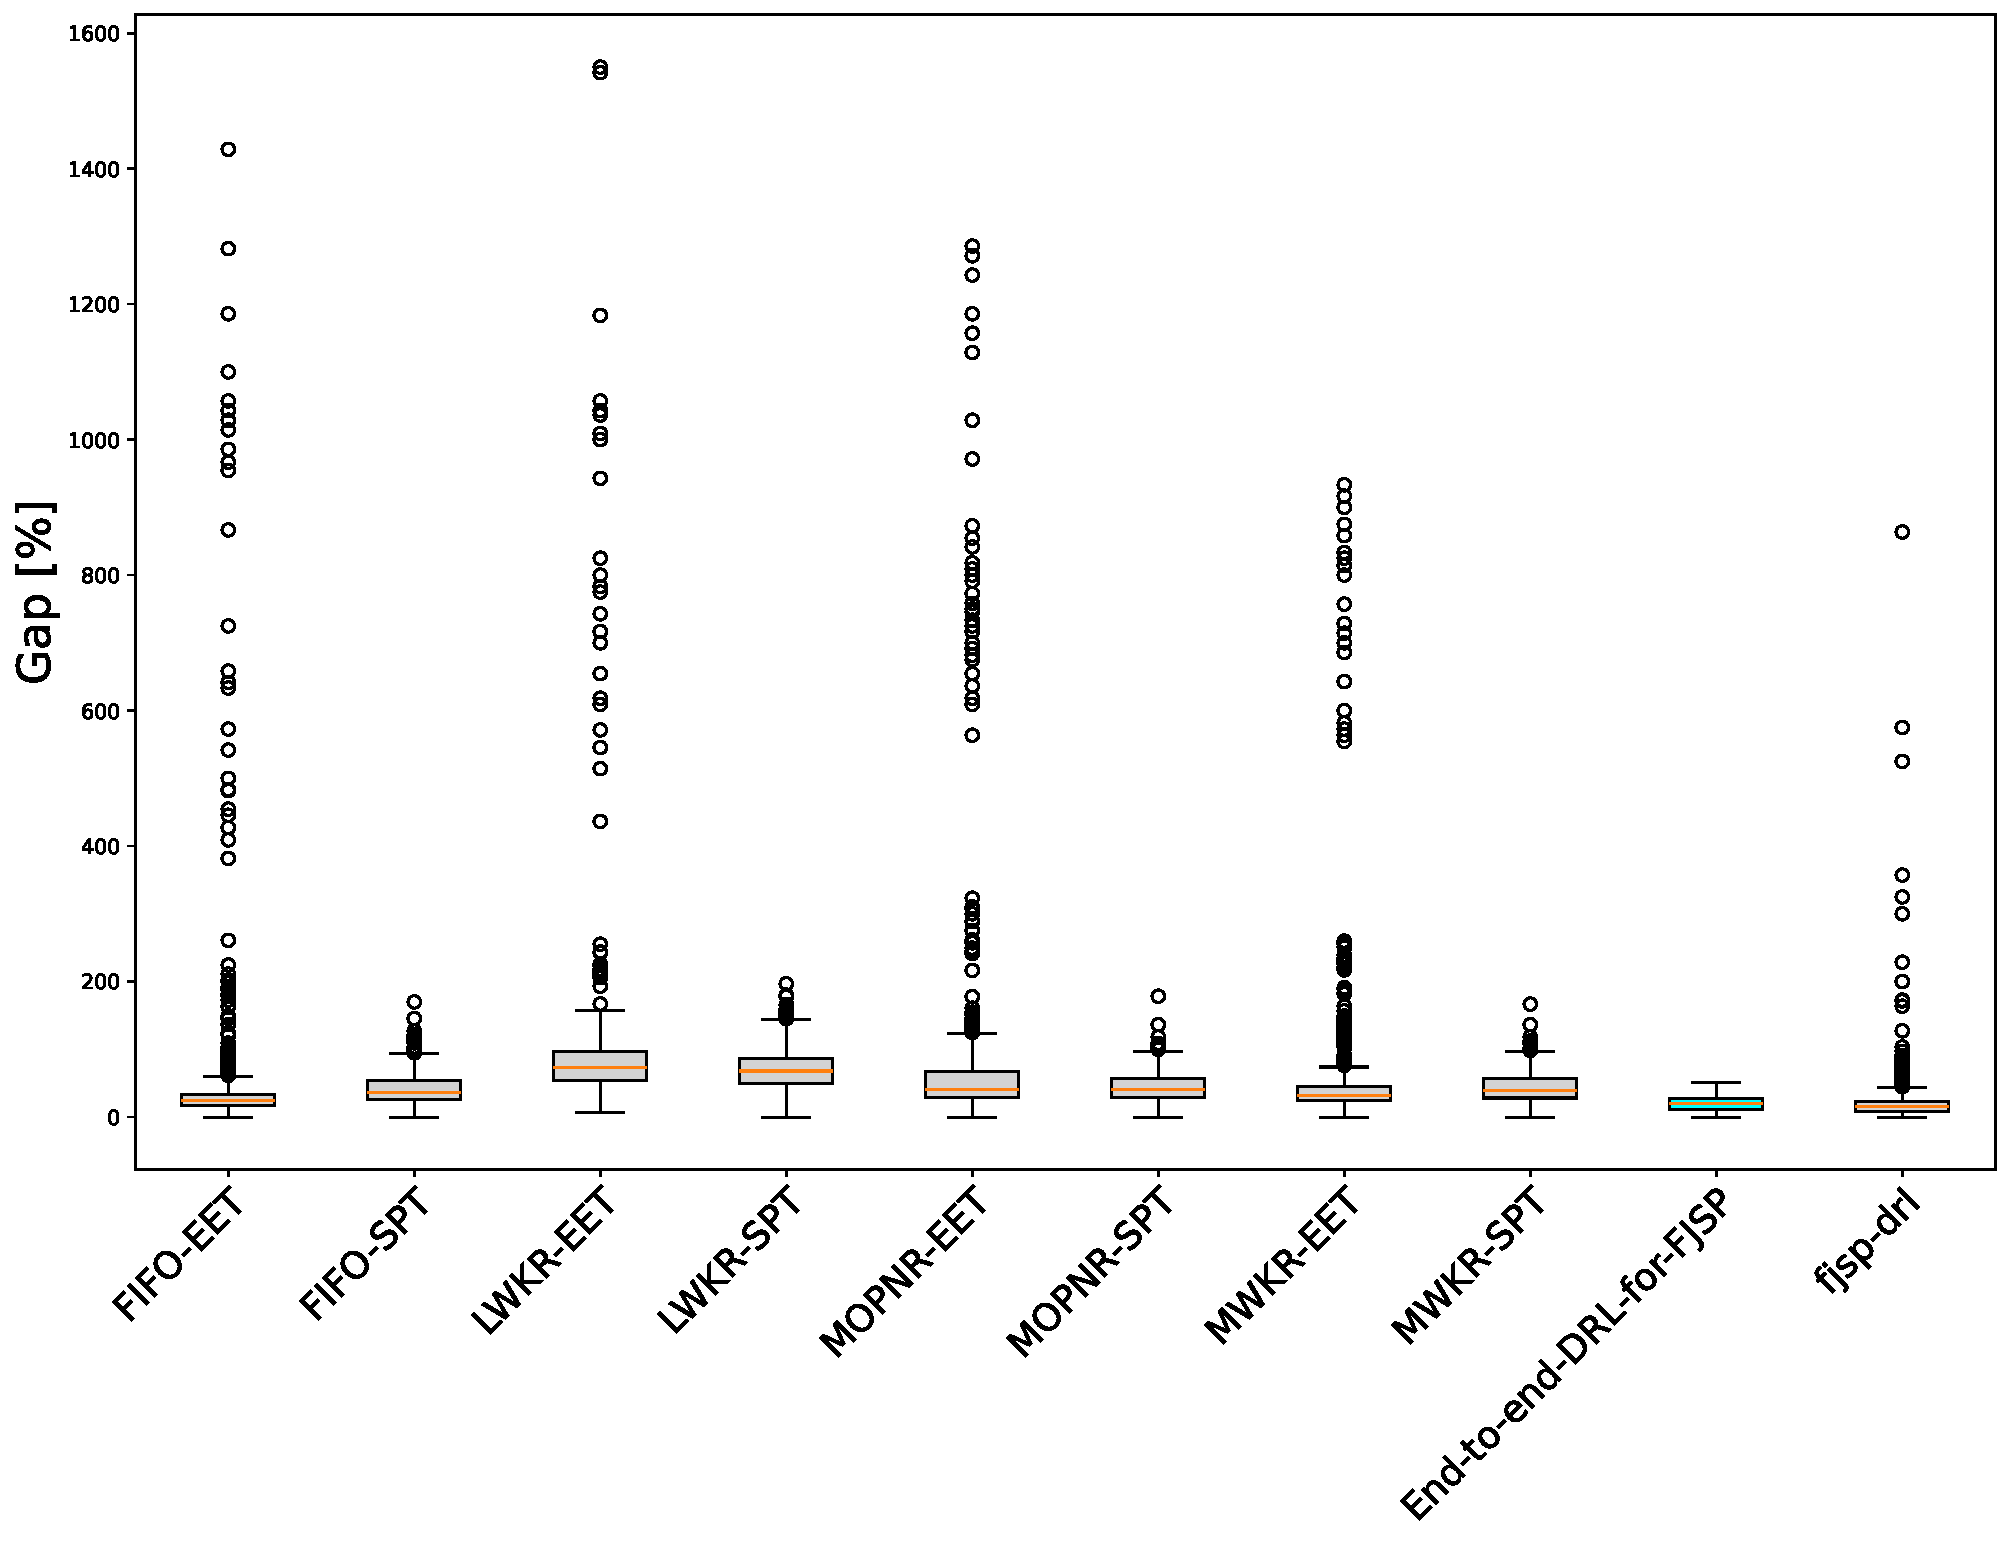
\includegraphics[width=0.8\linewidth]{images/horizontal_boxplot_fjsp_small.pdf}\\
    Figure 4.5: FJSP gaps for small instances
\end{center}

\begin{center}
    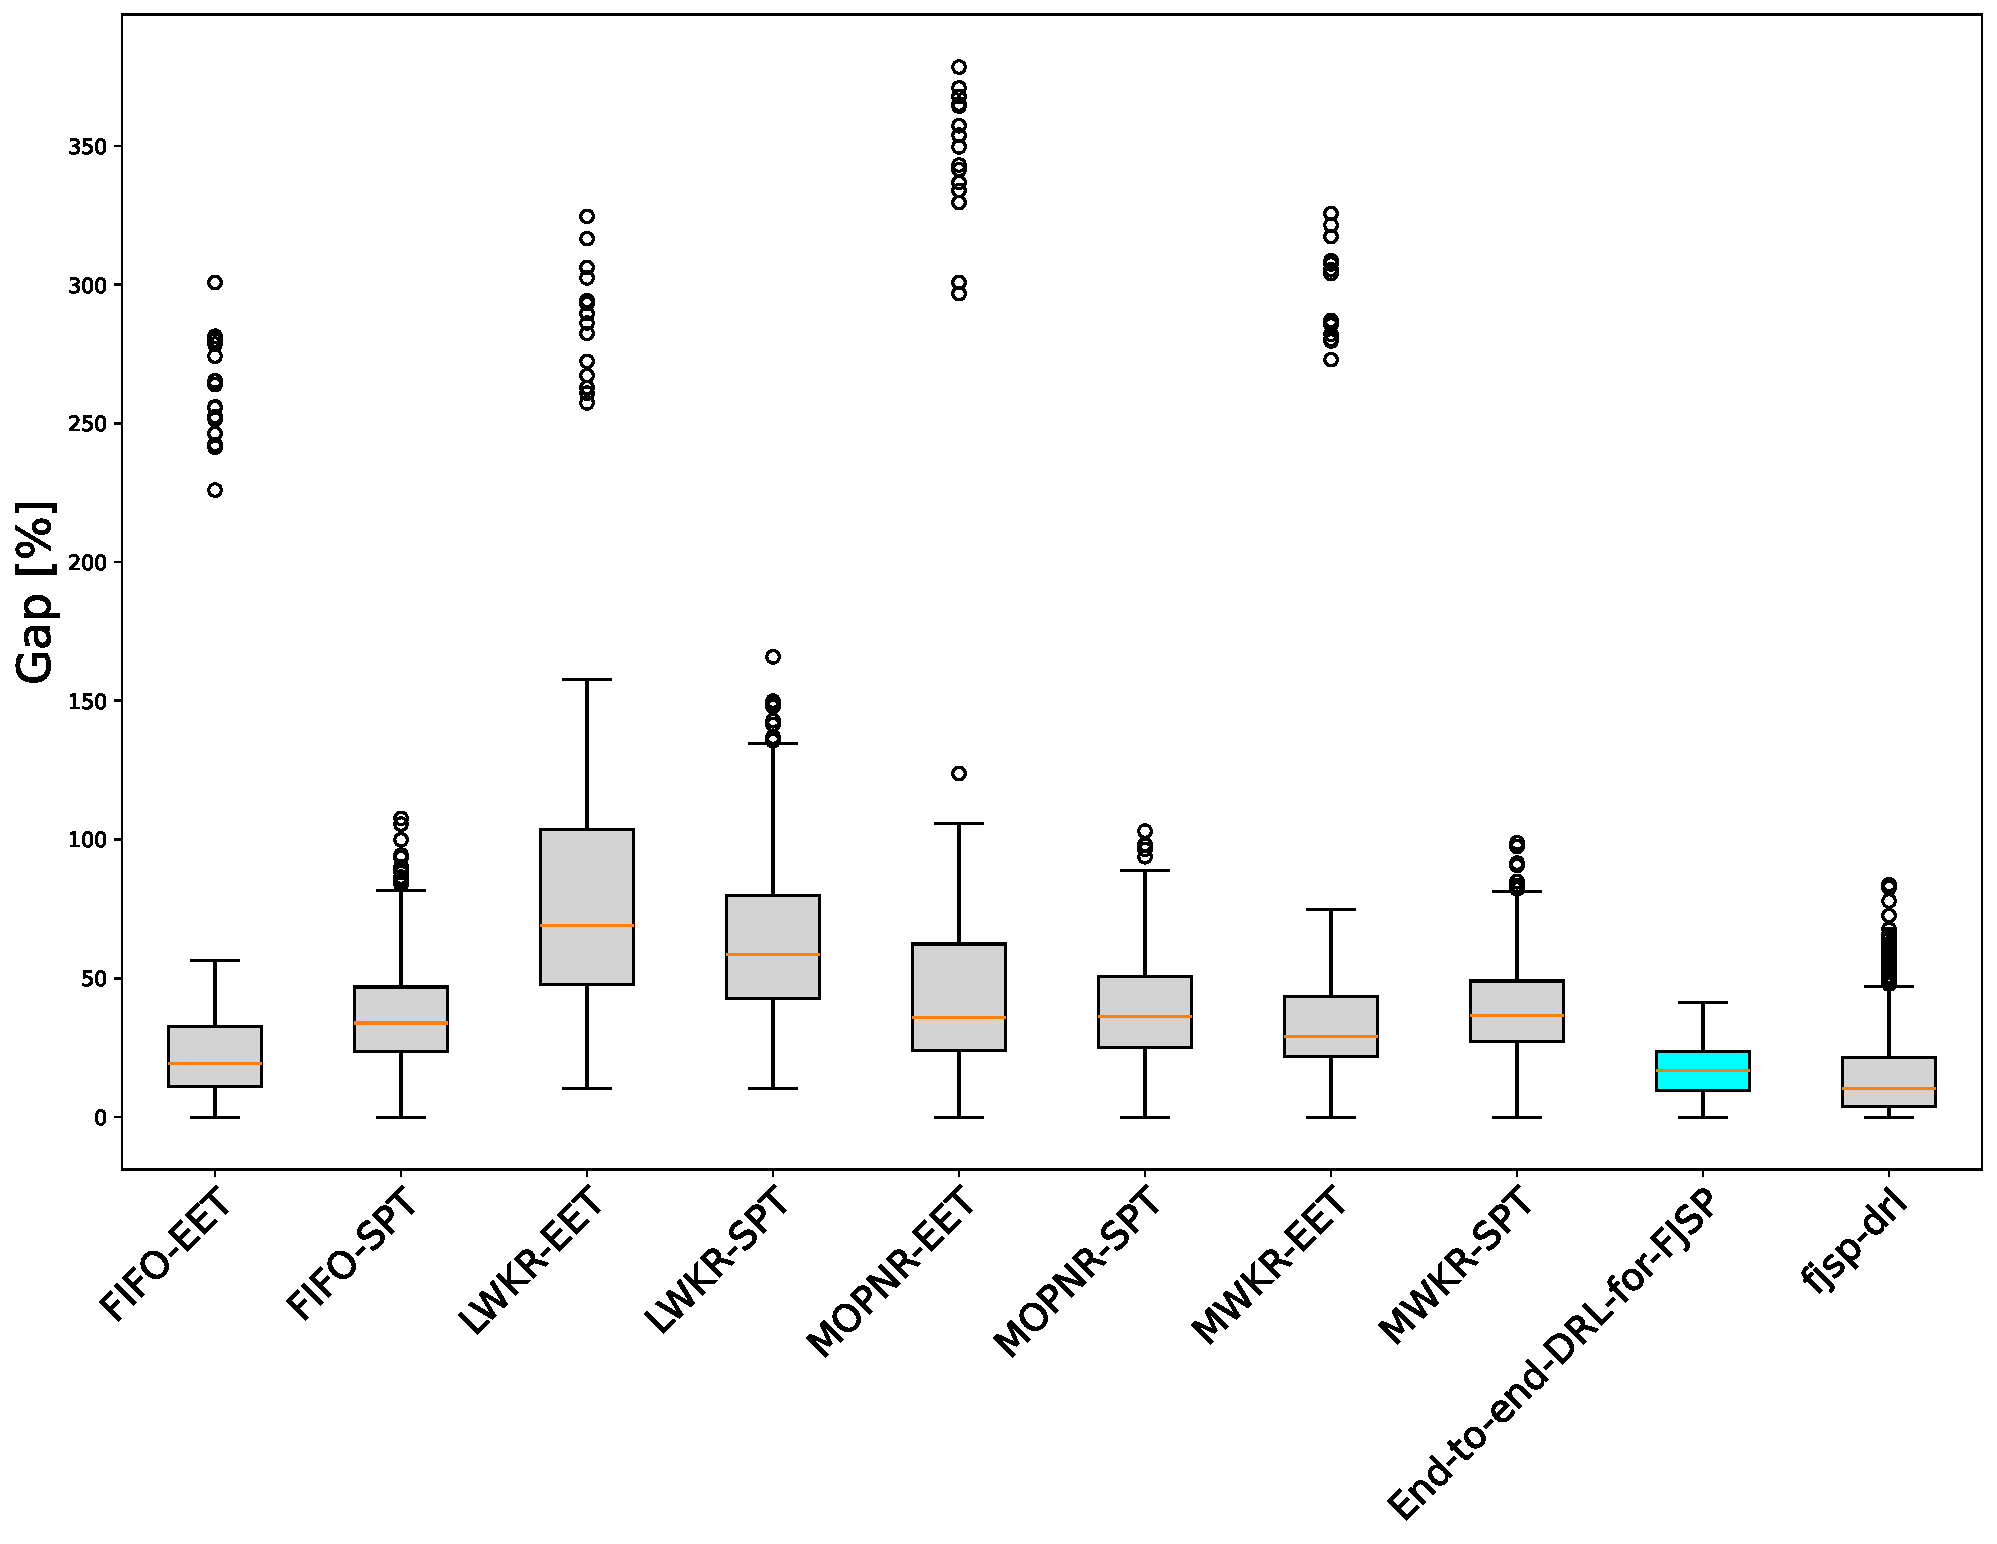
\includegraphics[width=0.8\linewidth]{images/horizontal_boxplot_fjsp_medium.pdf}\\
    Figure 4.6: FJSP gaps for medium instances
\end{center}
\begin{center}
    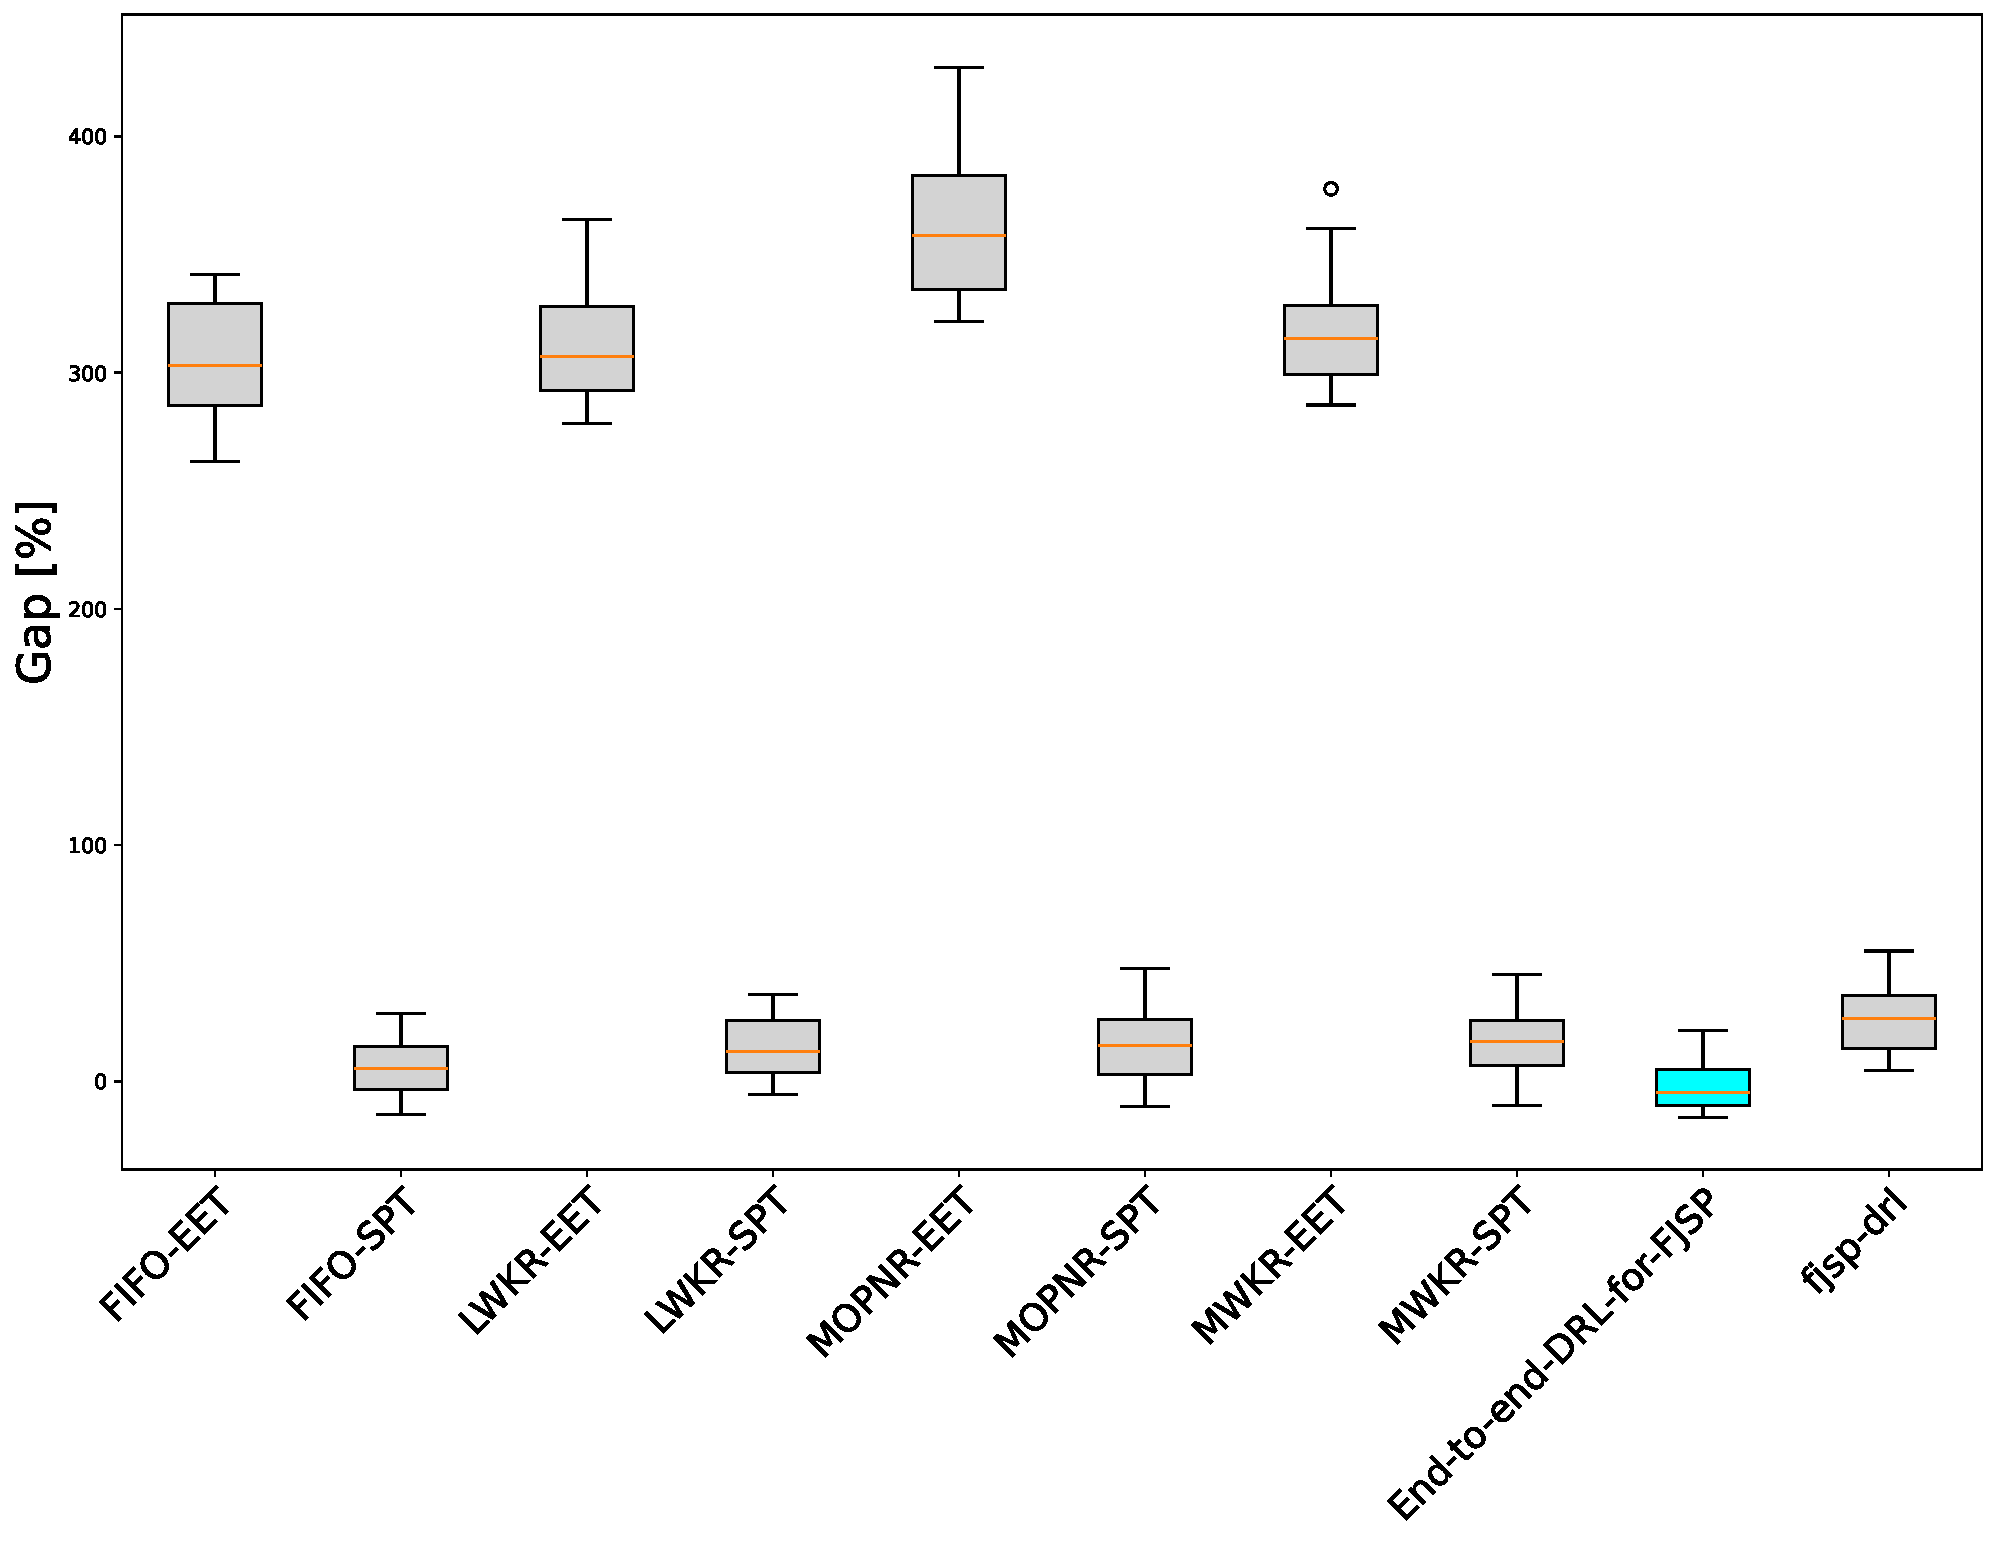
\includegraphics[width=0.8\linewidth]{images/horizontal_boxplot_fjsp_large.pdf}\\
    Figure 4.7: FJSP gaps for large instances
\end{center}
\begin{center}
    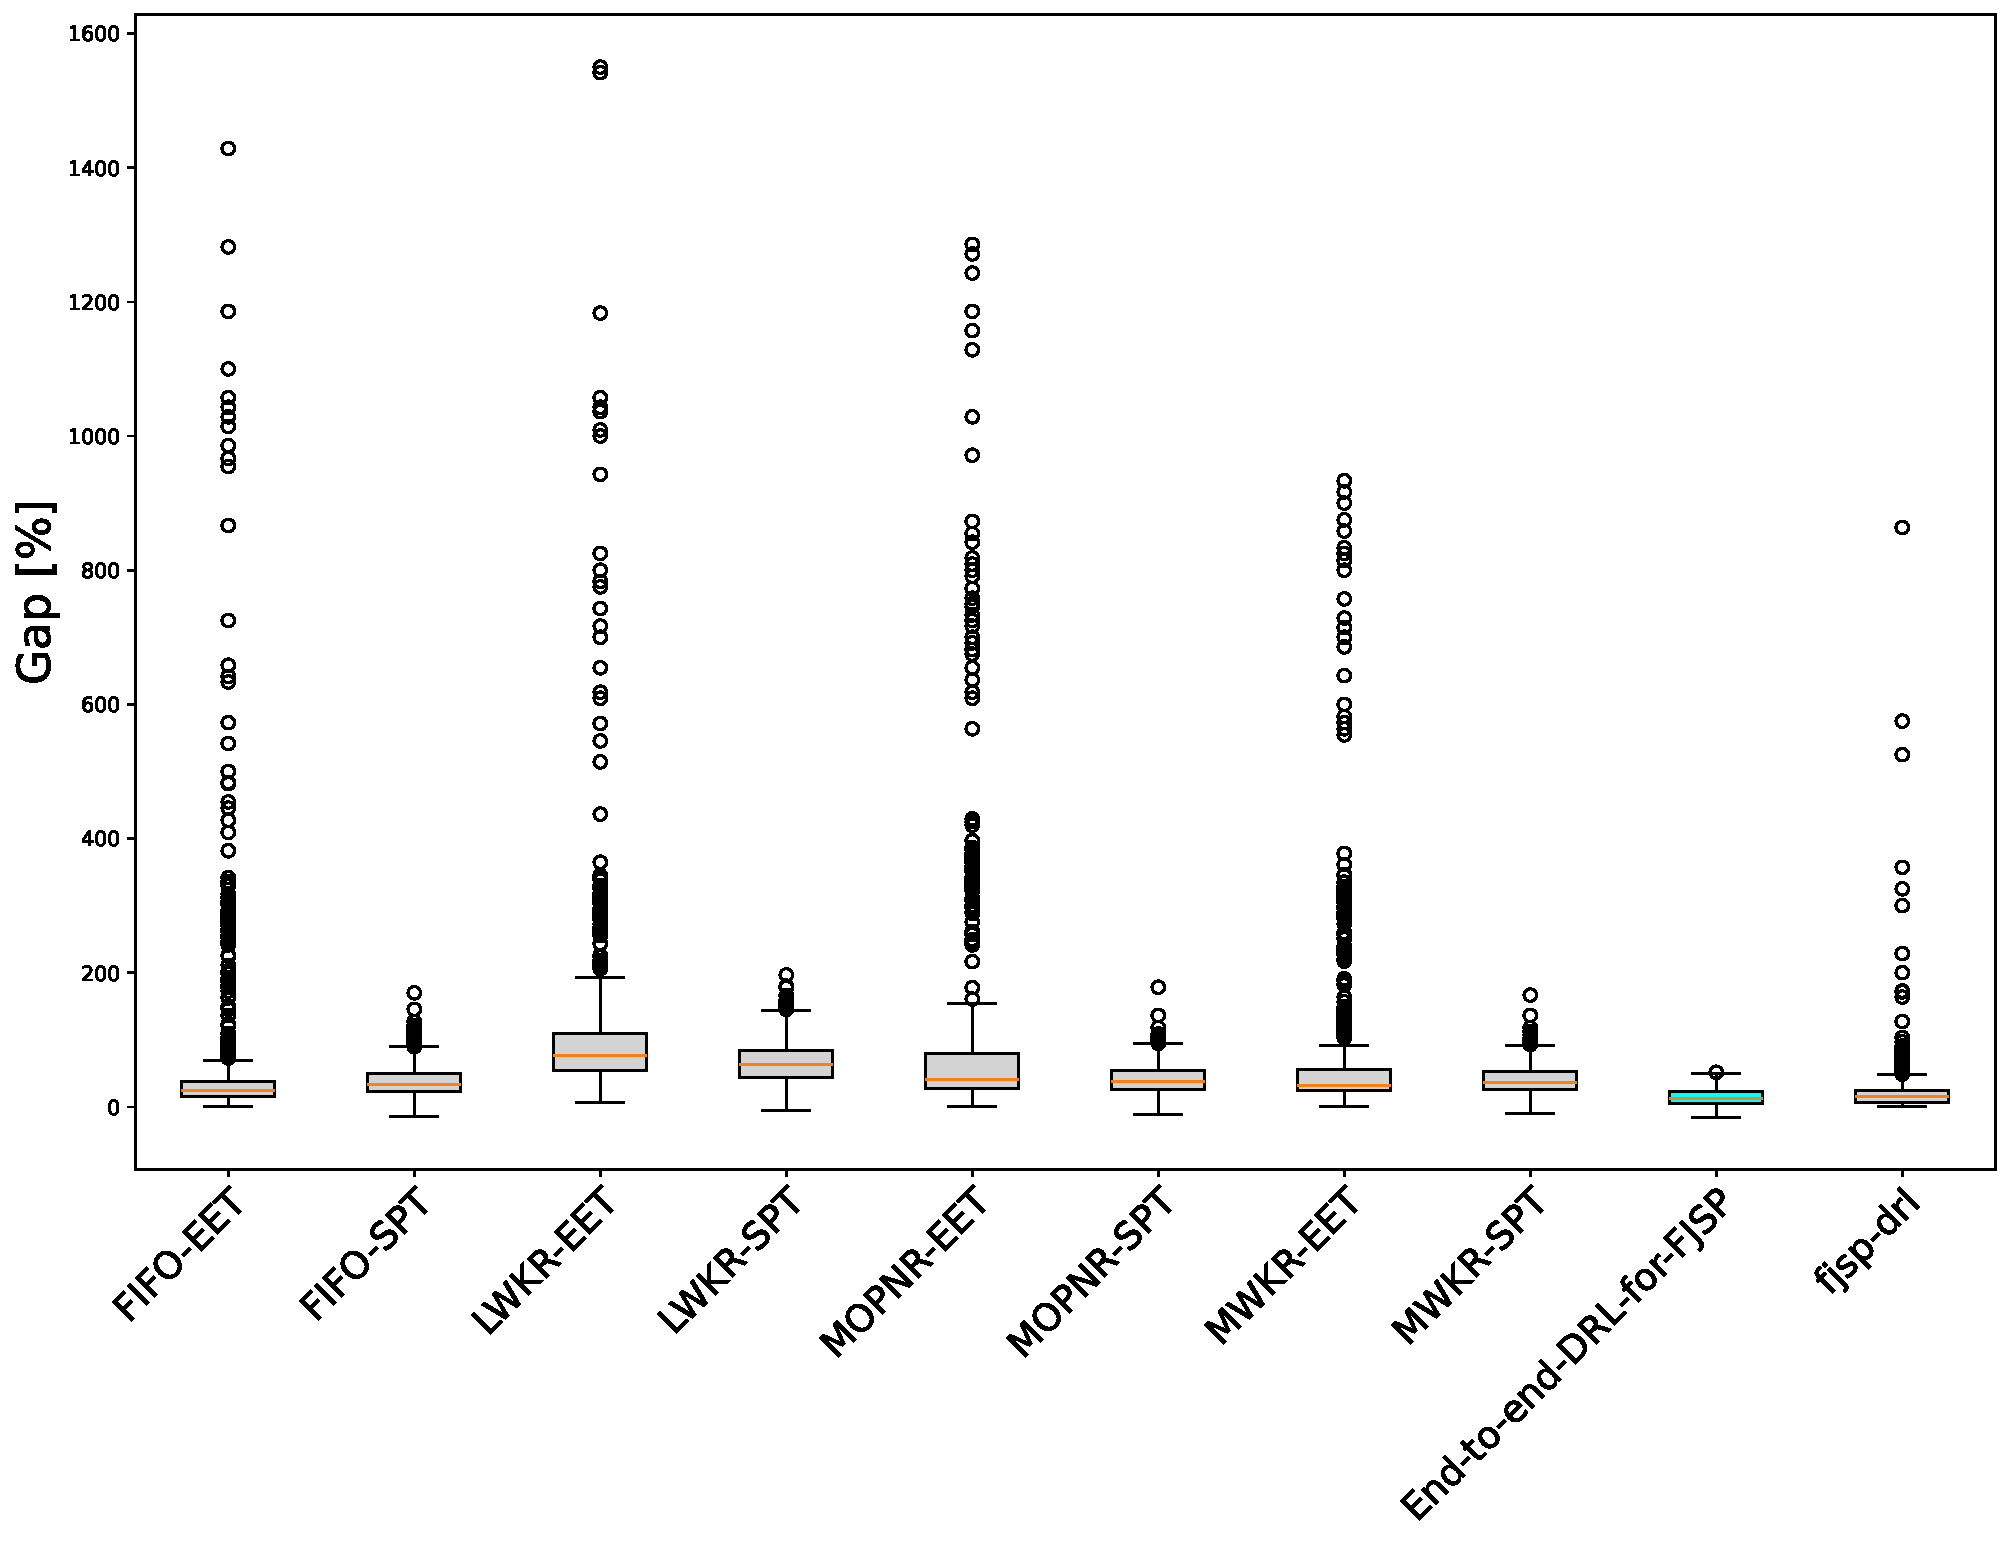
\includegraphics[width=0.8\linewidth]{images/horizontal_boxplot_fjsp_all.pdf}\\
    Figure 4.8: FJSP gaps for all instances
\end{center}

We tested the null hypothesis that the median values of gaps of all models and PDRs are from the same population using the Kruskal-Wallis test. The p-value is less than 1$\%$. Therefore, we reject this hypothesis. We also tested the null hypothesis that models \textbf{End-to-end-DRL-for-FJSP} and \textbf{fjsp-drl} are equal. The p-value was less than $1\%$ for small, medium, large, and all instances. Therefore, we rejected this null hypothesis.

\subsection{DJSP}

For DJSP, we don't have any upper bound available and can't compute the gap. Therefore, we will compare absolute makespans produced by different models for each size and load factor. Average DJSP makespans with load factor 1 are shown in Table 4.5, with load factor 2 in Table 4.6, and with load factor 4 in Table 4.7. The model with the smallest average makespan is highlighted in bold. For each size and load factor, we also tested the null hypothesis, which is that all models are equal. The corresponding p-values are also shown in each table.

\begin{table}
    Table 4.6: Average DJSP makespan with load factor 1\\
    \vspace{1mm}
    \label{table:4.6}
    \footnotesize 
    \begin{tabular}{ccccc}
        \toprule
        Size & L2D & IEEE-ICCE-RL-JSP & Wheatley & p-value \\
        \midrule
        6x6 & \textbf{72.03 ± 9.40} & 74.69 ± 11.38 & 77.00 ± 9.24 & 22.0$\%$ \\
        10x5 & \textbf{780.24 ± 90.34} & 874.43 ± 153.79 & 817.90 ± 78.99 & $< 1\%$ \\
        10x10 & \textbf{1204.43 ± 219.98} & 1259.91 ± 257.09 & 1212.22 ± 217.04 & $< 1\%$ \\
        15x5 & \textbf{1031.16 ± 61.63} & 1198.84 ± 108.35 & 1080.24 ± 89.20 & $< 1\%$ \\
        15x10 & \textbf{1329.93 ± 94.21} & 1413.15 ± 116.03 & 1442.65 ± 129.44 & $< 1\%$ \\
        15x15 & \textbf{1676.67 ± 116.37} & 1716.56 ± 119.06 & 1817.81 ± 145.40 & $< 1\%$ \\
        20x5 & \textbf{1363.52 ± 148.91} & 1701.57 ± 203.56 & 1367.97 ± 104.40 & $< 1\%$ \\
        20x10 & \textbf{1858.25 ± 213.24} & 2081.56 ± 257.26 & 1918.04 ± 161.88 & $< 1\%$ \\
        20x15 & \textbf{2779.05 ± 1270.01} & 3009.12 ± 1383.13 & 2988.77 ± 1338.80 & $< 1\%$ \\
        20x20 & \textbf{3208.98 ± 1522.30} & 3402.65 ± 1637.48 & 3655.56 ± 1662.28 & $< 1\%$ \\
        30x10 & \textbf{2143.03 ± 126.54} & 2511.60 ± 222.45 & 2510.66 ± 181.78 & $< 1\%$ \\
        30x15 & \textbf{4034.07 ± 1660.43} & 4484.68 ± 1833.57 & 4819.48 ± 1847.26 & $< 1\%$ \\
        30x20 & \textbf{4469.95 ± 1779.81} & 4844.21 ± 1961.36 & 5805.12 ± 2149.98 & $< 1\%$ \\
        40x15 & \textbf{6835.81 ± 1080.76} & 7789.19 ± 1137.65 & 8884.73 ± 862.80 & $< 1\%$ \\
        40x20 & \textbf{7556.13 ± 1071.72} & 8496.36 ± 1179.83 & 10985.64 ± 1032.40 & $< 1\%$ \\
        50x10 & \textbf{3809.08 ± 766.24} & 4456.46 ± 684.34 & 4948.68 ± 604.10 & $< 1\%$ \\
        50x15 & \textbf{5882.77 ± 2621.21} & 6689.03 ± 2736.00 & 9118.45 ± 3524.75 & $< 1\%$ \\
        50x20 & \textbf{6320.83 ± 2770.31} & 7050.68 ± 3024.71 & 11367.83 ± 4334.55 & $< 1\%$ \\
        100x20 & \textbf{6310.22 ± 178.01} & 8150.22 ± 347.98 & 22838.04 ± 1550.05 & $< 1\%$ \\
        \bottomrule
    \end{tabular}
\end{table}
    
\begin{table}
    Table 4.7: Average DJSP makespan with load factor 2\\
    \vspace{1mm}
    \label{table:4.7}
    \footnotesize 
    \begin{tabular}{ccccc}
    \toprule
    Size & L2D & IEEE-ICCE-RL-JSP & Wheatley & p-value \\
    \midrule
    6x6 & 70.47 ± 8.20 & \textbf{67.65 ± 7.26} & 76.67 ± 6.82 & 1.0$\%$ \\
    10x5 & \textbf{755.77 ± 83.86} & 782.58 ± 101.48 & 792.24 ± 71.32 & $< 1\%$ \\
    10x10 & 1189.79 ± 216.81 & \textbf{1157.23 ± 214.02} & 1190.19 ± 215.12 & $< 1\%$ \\
    15x5 & \textbf{1006.95 ± 55.52} & 1045.68 ± 63.48 & 1027.94 ± 70.34 & $< 1\%$ \\
    15x10 & 1287.60 ± 92.94 & \textbf{1261.18 ± 81.78} & 1352.46 ± 97.29 & $< 1\%$ \\
    15x15 & 1620.90 ± 99.44 & \textbf{1567.52 ± 81.21} & 1723.14 ± 114.35 & $< 1\%$ \\
    20x5 & 1345.86 ± 175.94 & 1453.60 ± 147.46 & \textbf{1334.19 ± 115.78} & $< 1\%$ \\
    20x10 & 1843.55 ± 254.44 & \textbf{1819.53 ± 224.32} & 1865.27 ± 199.47 & 8.0$\%$ \\
    20x15 & 2711.67 ± 1266.34 & \textbf{2672.22 ± 1241.38} & 2873.04 ± 1324.80 & $< 1\%$ \\
    20x20 & 3101.05 ± 1513.44 & \textbf{3059.03 ± 1483.54} & 3487.31 ± 1644.74 & $< 1\%$ \\
    30x10 & \textbf{2066.74 ± 112.36} & 2155.90 ± 129.13 & 2290.94 ± 143.52 & $< 1\%$ \\
    30x15 & 3980.79 ± 1722.64 & \textbf{3976.93 ± 1644.38} & 4503.40 ± 1835.45 & $< 1\%$ \\
    30x20 & 4365.50 ± 1814.25 & \textbf{4335.11 ± 1776.02} & 5335.82 ± 2091.11 & $< 1\%$ \\
    40x15 & \textbf{6792.66 ± 1268.41} & 6872.78 ± 1083.83 & 8185.63 ± 1053.13 & $< 1\%$ \\
    40x20 & \textbf{7478.68 ± 1261.55} & 7541.90 ± 1112.00 & 10009.41 ± 1058.23 & $< 1\%$ \\
    50x10 & \textbf{3852.59 ± 847.80} & 3920.64 ± 658.72 & 4468.24 ± 702.64 & $< 1\%$ \\
    50x15 & \textbf{5842.31 ± 2704.56} & 5887.95 ± 2467.82 & 7981.61 ± 3227.05 & $< 1\%$ \\
    50x20 & \textbf{6249.35 ± 2860.16} & 6276.52 ± 2763.67 & 10040.22 ± 3978.86 & $< 1\%$ \\
    100x20 & \textbf{6129.85 ± 201.99} & 6858.02 ± 240.68 & 19085.54 ± 1326.74 & $< 1\%$ \\
    \bottomrule
    \end{tabular}
\end{table}
    
\begin{table}
    Table 4.8: Average DJSP makespan with load factor 4\\
    \vspace{1mm}
    \label{table:4.8}
    \footnotesize 
    \begin{tabular}{ccccc}
    \toprule
    Size & L2D & IEEE-ICCE-RL-JSP & Wheatley & p-value \\
    \midrule
    6x6 & 70.05 ± 8.25 & \textbf{64.48 ± 3.84} & 75.50 ± 8.55 & $< 1\%$ \\
    10x5 & 747.63 ± 75.82 & \textbf{741.80 ± 78.28} & 775.62 ± 77.70 & 2.0$\%$ \\
    10x10 & 1176.08 ± 221.28 & \textbf{1109.18 ± 200.95} & 1187.33 ± 212.06 & $< 1\%$ \\
    15x5 & 1006.18 ± 53.37 & \textbf{984.55 ± 44.94} & 1008.57 ± 61.81 & $< 1\%$ \\
    15x10 & 1274.83 ± 76.31 & \textbf{1191.63 ± 70.89} & 1321.84 ± 85.92 & $< 1\%$ \\
    15x15 & 1598.28 ± 96.13 & \textbf{1506.20 ± 70.61} & 1681.24 ± 97.81 & $< 1\%$ \\
    20x5 & 1343.42 ± 184.64 & 1339.17 ± 134.68 & \textbf{1333.13 ± 131.26} & 67.0$\%$ \\
    20x10 & 1835.01 ± 272.46 & \textbf{1710.64 ± 218.77} & 1868.15 ± 233.91 & $< 1\%$ \\
    20x15 & 2695.64 ± 1268.49 & \textbf{2541.11 ± 1179.87} & 2852.97 ± 1325.87 & $< 1\%$ \\
    20x20 & 3066.77 ± 1509.04 & \textbf{2902.33 ± 1419.60} & 3446.61 ± 1688.14 & $< 1\%$ \\
    30x10 & 2036.46 ± 114.04 & \textbf{1993.52 ± 92.45} & 2207.02 ± 132.10 & $< 1\%$ \\
    30x15 & 3955.84 ± 1730.05 & \textbf{3742.95 ± 1567.90} & 4412.12 ± 1870.05 & $< 1\%$ \\
    30x20 & 4330.06 ± 1818.44 & \textbf{4122.12 ± 1719.04} & 5214.83 ± 2106.46 & $< 1\%$ \\
    40x15 & 6757.92 ± 1322.93 & \textbf{6408.27 ± 1070.14} & 7954.02 ± 1196.00 & $< 1\%$ \\
    40x20 & 7463.87 ± 1319.68 & \textbf{7114.58 ± 1091.71} & 9642.57 ± 1169.56 & $< 1\%$ \\
    50x10 & 3885.63 ± 873.73 & \textbf{3676.22 ± 659.45} & 4241.08 ± 729.50 & $< 1\%$ \\
    50x15 & 5810.45 ± 2723.58 & \textbf{5504.96 ± 2345.68} & 7504.37 ± 3180.44 & $< 1\%$ \\
    50x20 & 6227.76 ± 2894.36 & \textbf{5883.56 ± 2631.55} & 9320.83 ± 3888.32 & $< 1\%$ \\
    100x20 & \textbf{6076.26 ± 226.25} & 6225.12 ± 206.62 & 16734.28 ± 1051.45 & $< 1\%$ \\
    \bottomrule
    \end{tabular}
\end{table}
    
We can reject the null hypothesis for almost all sizes and load factors. We also tested the null hypothesis for each load factor and instance size, that the pair of models are equal using the Mann-Whitney \textit{U} test. The majority of instance sizes and load factors had p-value $< 5\%$, and thus, we rejected the null hypothesis for them. Cases, where we could not reject the null hypothesis, are shown in Table 4.8.

\begin{table}
    Table 4.9: DJSP cases without rejected null hypothesis\\
    \vspace{1mm}
    \label{table:4.9}
    \begin{tabular}{ccccc}
        \toprule
        Size & Load factor & First model & Second model & p-value \\
        \midrule
        6x6 & 1 & IEEE-ICCE-RL-JSP & L2D & 33.0$\%$ \\
        6x6 & 1 & IEEE-ICCE-RL-JSP & Wheatley & 32.0$\%$ \\
        6x6 & 1 & L2D & Wheatley & 11.0$\%$ \\
        6x6 & 2 & IEEE-ICCE-RL-JSP & L2D & 22.0$\%$ \\
        6x6 & 4 & L2D & Wheatley & 8.0$\%$ \\
        10x5 & 2 & IEEE-ICCE-RL-JSP & Wheatley & 34.0$\%$ \\
        10x5 & 4 & IEEE-ICCE-RL-JSP & L2D & 58.0$\%$ \\
        10x10 & 1 & L2D & Wheatley & 65.0$\%$ \\
        10x10 & 2 & L2D & Wheatley & 91.0$\%$ \\
        10x10 & 4 & L2D & Wheatley & 59.0$\%$ \\
        15x5 & 4 & L2D & Wheatley & 76.0$\%$ \\
        15x10 & 1 & IEEE-ICCE-RL-JSP & Wheatley & 12.0$\%$ \\
        20x5 & 1 & L2D & Wheatley & 42.0$\%$ \\
        20x5 & 2 & L2D & Wheatley & 64.0$\%$ \\
        20x5 & 4 & IEEE-ICCE-RL-JSP & L2D & 37.0$\%$ \\
        20x5 & 4 & IEEE-ICCE-RL-JSP & Wheatley & 94.0$\%$ \\
        20x5 & 4 & L2D & Wheatley & 79.0$\%$ \\
        20x10 & 2 & IEEE-ICCE-RL-JSP & L2D & 9.0$\%$ \\
        20x10 & 2 & L2D & Wheatley & 28.0$\%$ \\
        20x10 & 4 & L2D & Wheatley & 12.0$\%$ \\
        20x15 & 1 & IEEE-ICCE-RL-JSP & Wheatley & 78.0$\%$ \\
        20x15 & 2 & IEEE-ICCE-RL-JSP & L2D & 10.0$\%$ \\
        30x10 & 1 & IEEE-ICCE-RL-JSP & Wheatley & 64.0$\%$ \\
        30x15 & 2 & IEEE-ICCE-RL-JSP & L2D & 26.0$\%$ \\
        30x20 & 2 & IEEE-ICCE-RL-JSP & L2D & 16.0$\%$ \\
        40x15 & 2 & IEEE-ICCE-RL-JSP & L2D & 7.0$\%$ \\
        \bottomrule
        \end{tabular}        
\end{table}